\chapter{Components} 
\label{sec:components}

\begin{figure}[h!]
  \begin{center}
  {\subfigcapskip = 5pt \subfigcapmargin = -12pt \subfigure[]{\label{fig:edge-a}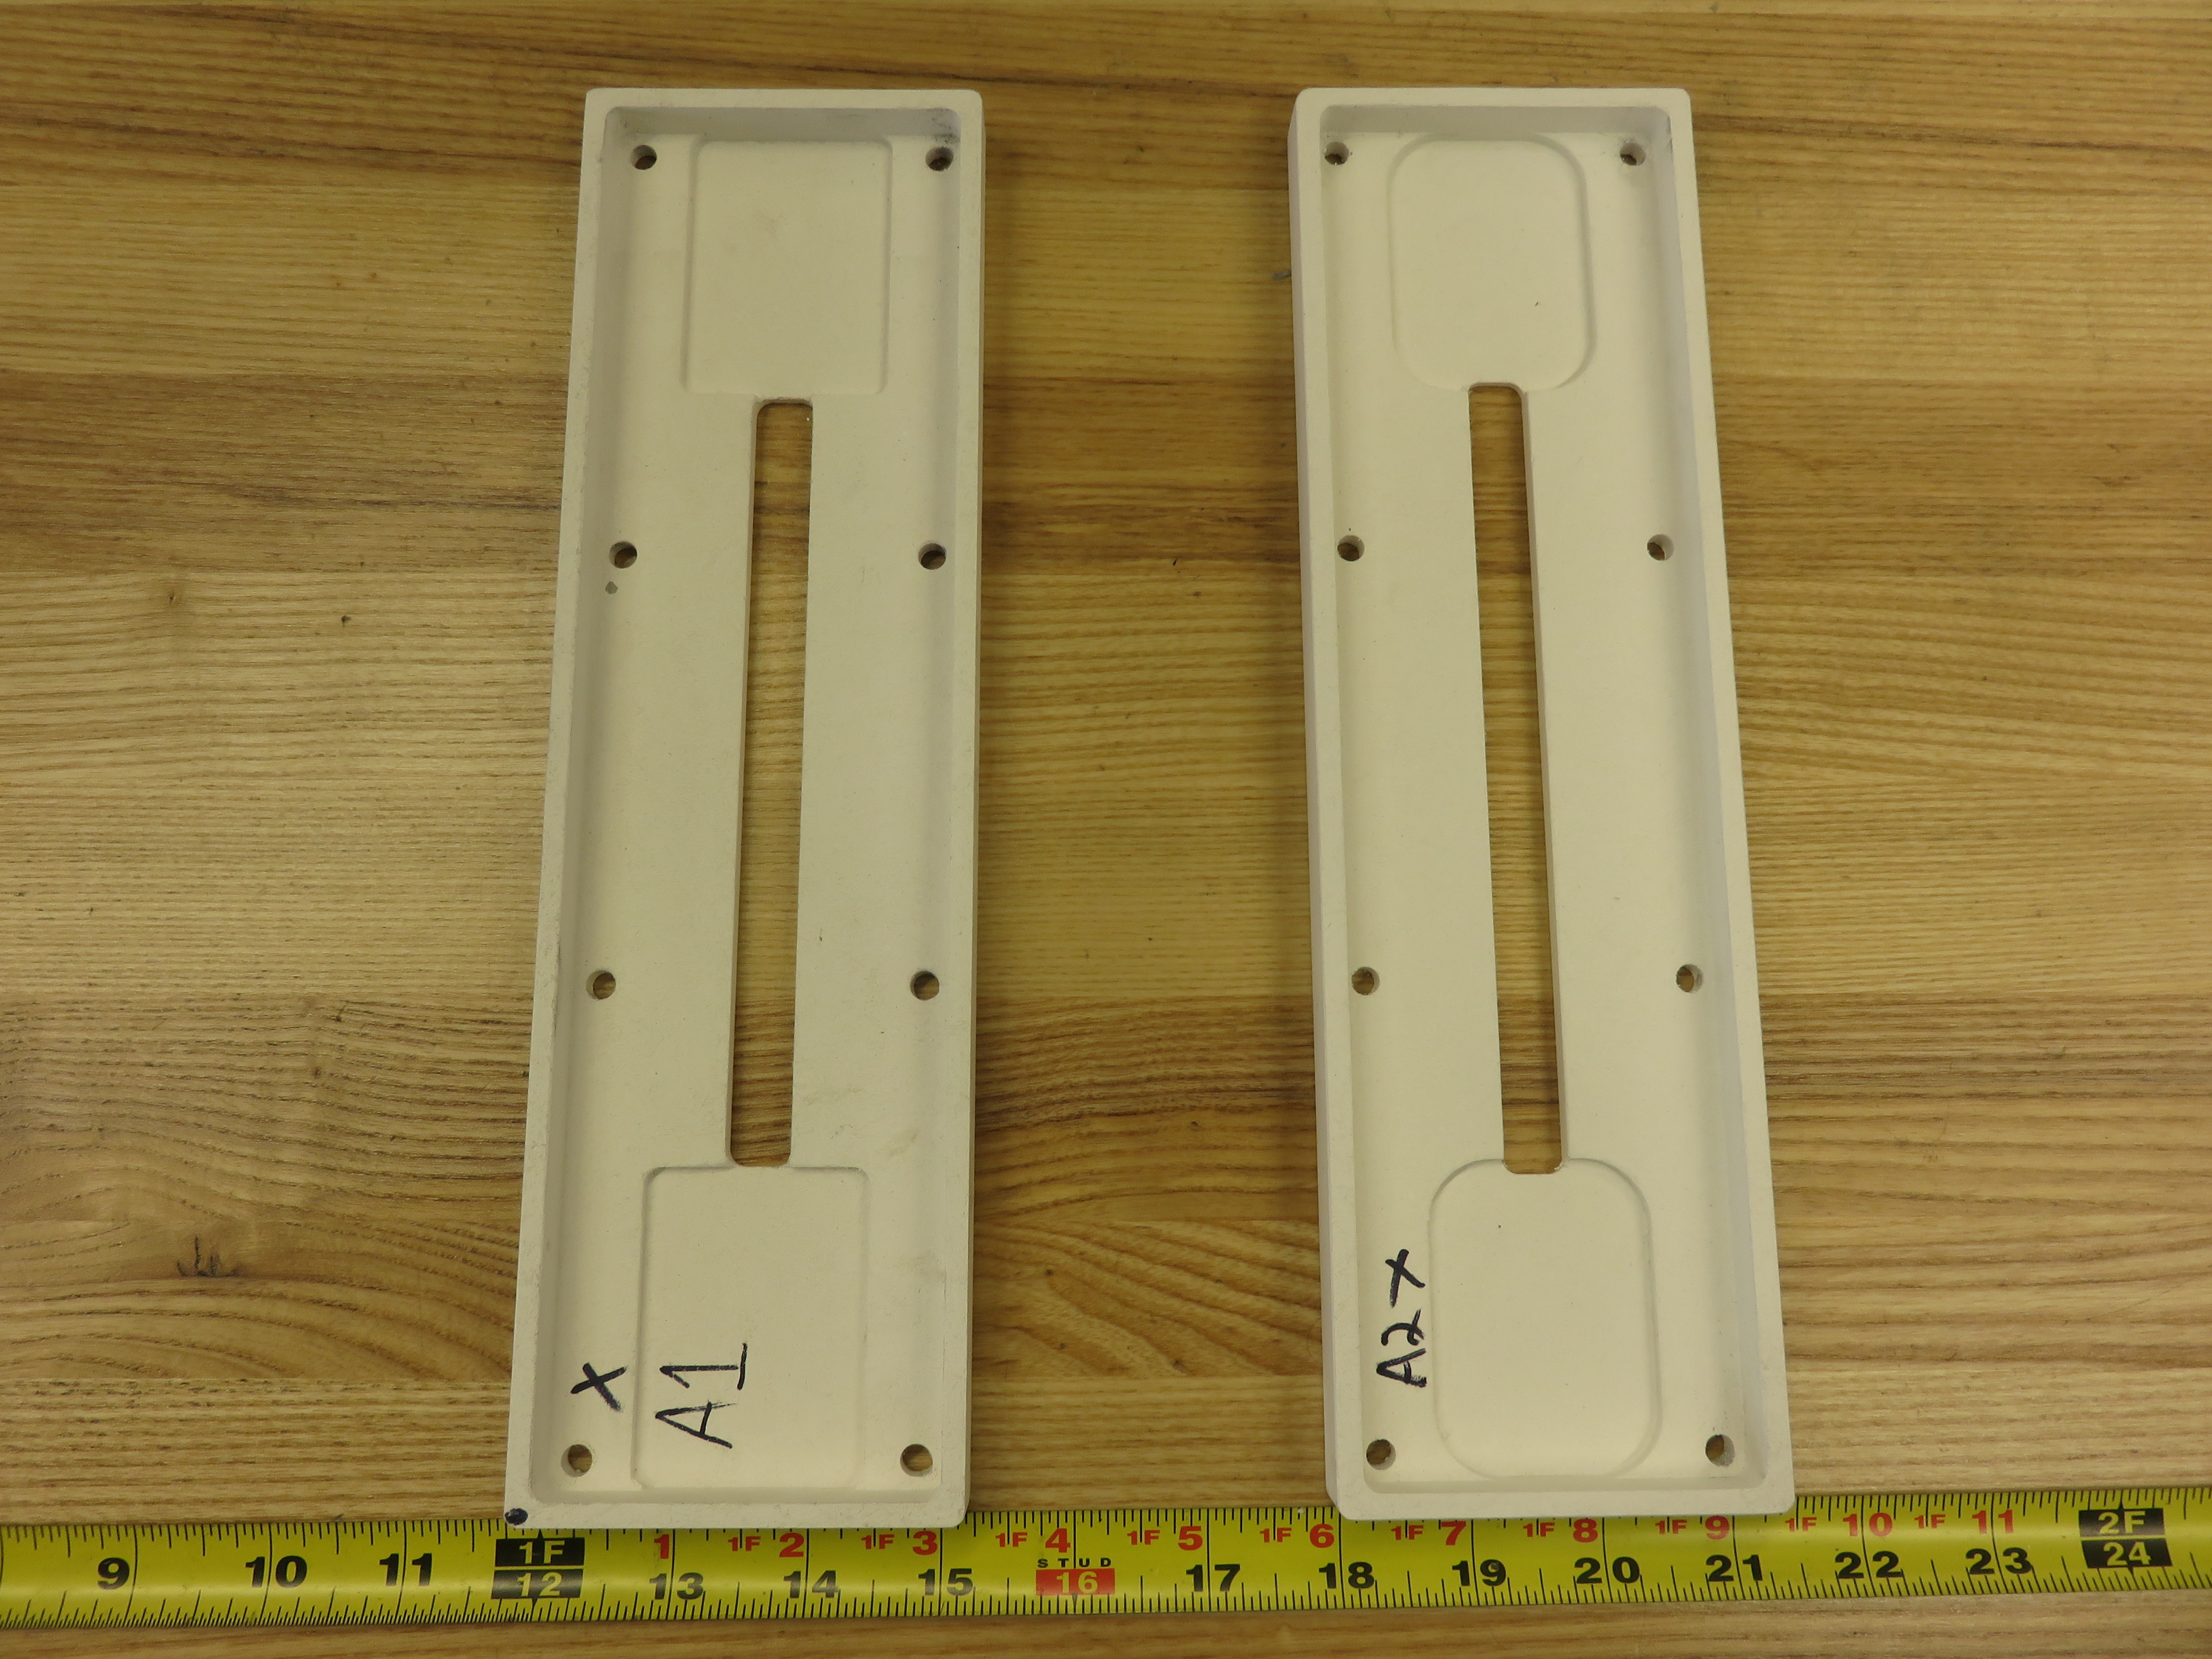
\includegraphics[scale=0.1]{facility/MachinedParts/A_insul_v2.JPG}}}
   {\subfigcapskip = 5pt \subfigcapmargin = -12pt  \subfigure[]{\label{fig:edge-b}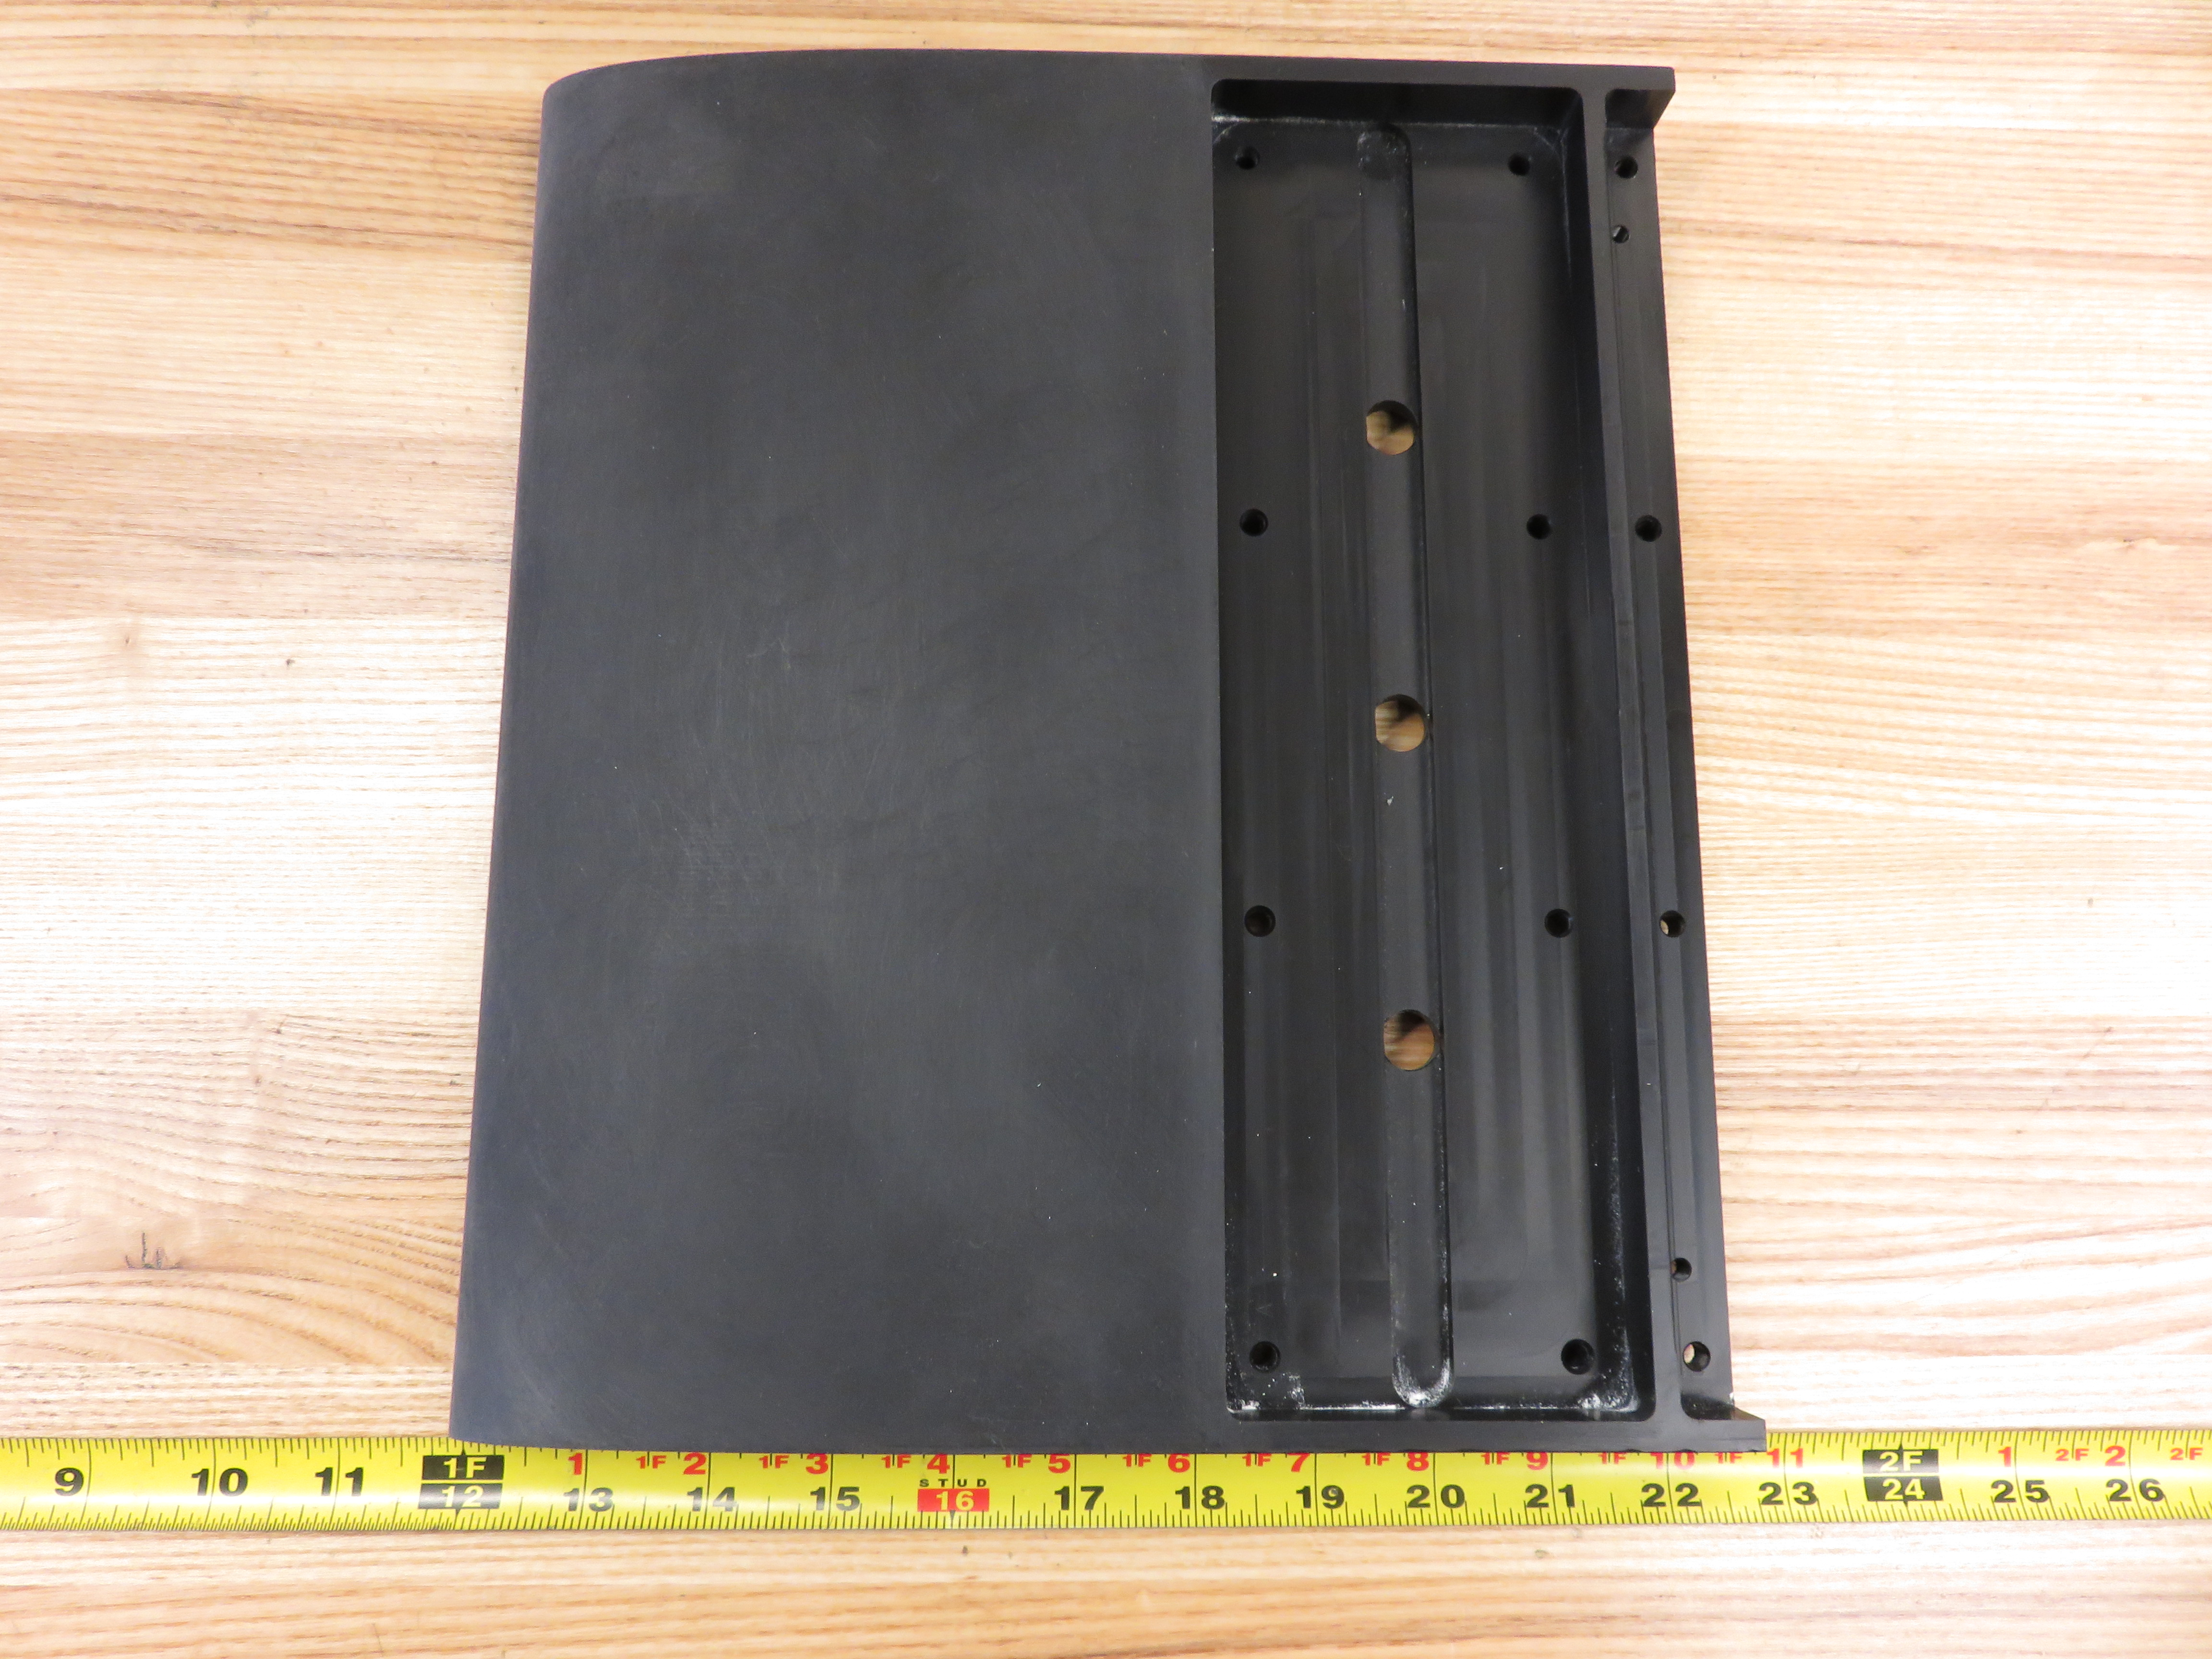
\includegraphics[scale=0.1]{facility/MachinedParts/A_meas_v2.JPG}}}
  \end{center}
\caption{(a) insulation (b) frame. } 
\label{fig:partsA}
\end{figure}

\begin{figure}[h!]
  \begin{center}
  {\subfigcapskip = 5pt \subfigcapmargin = -12pt \subfigure[]{\label{fig:edge-a}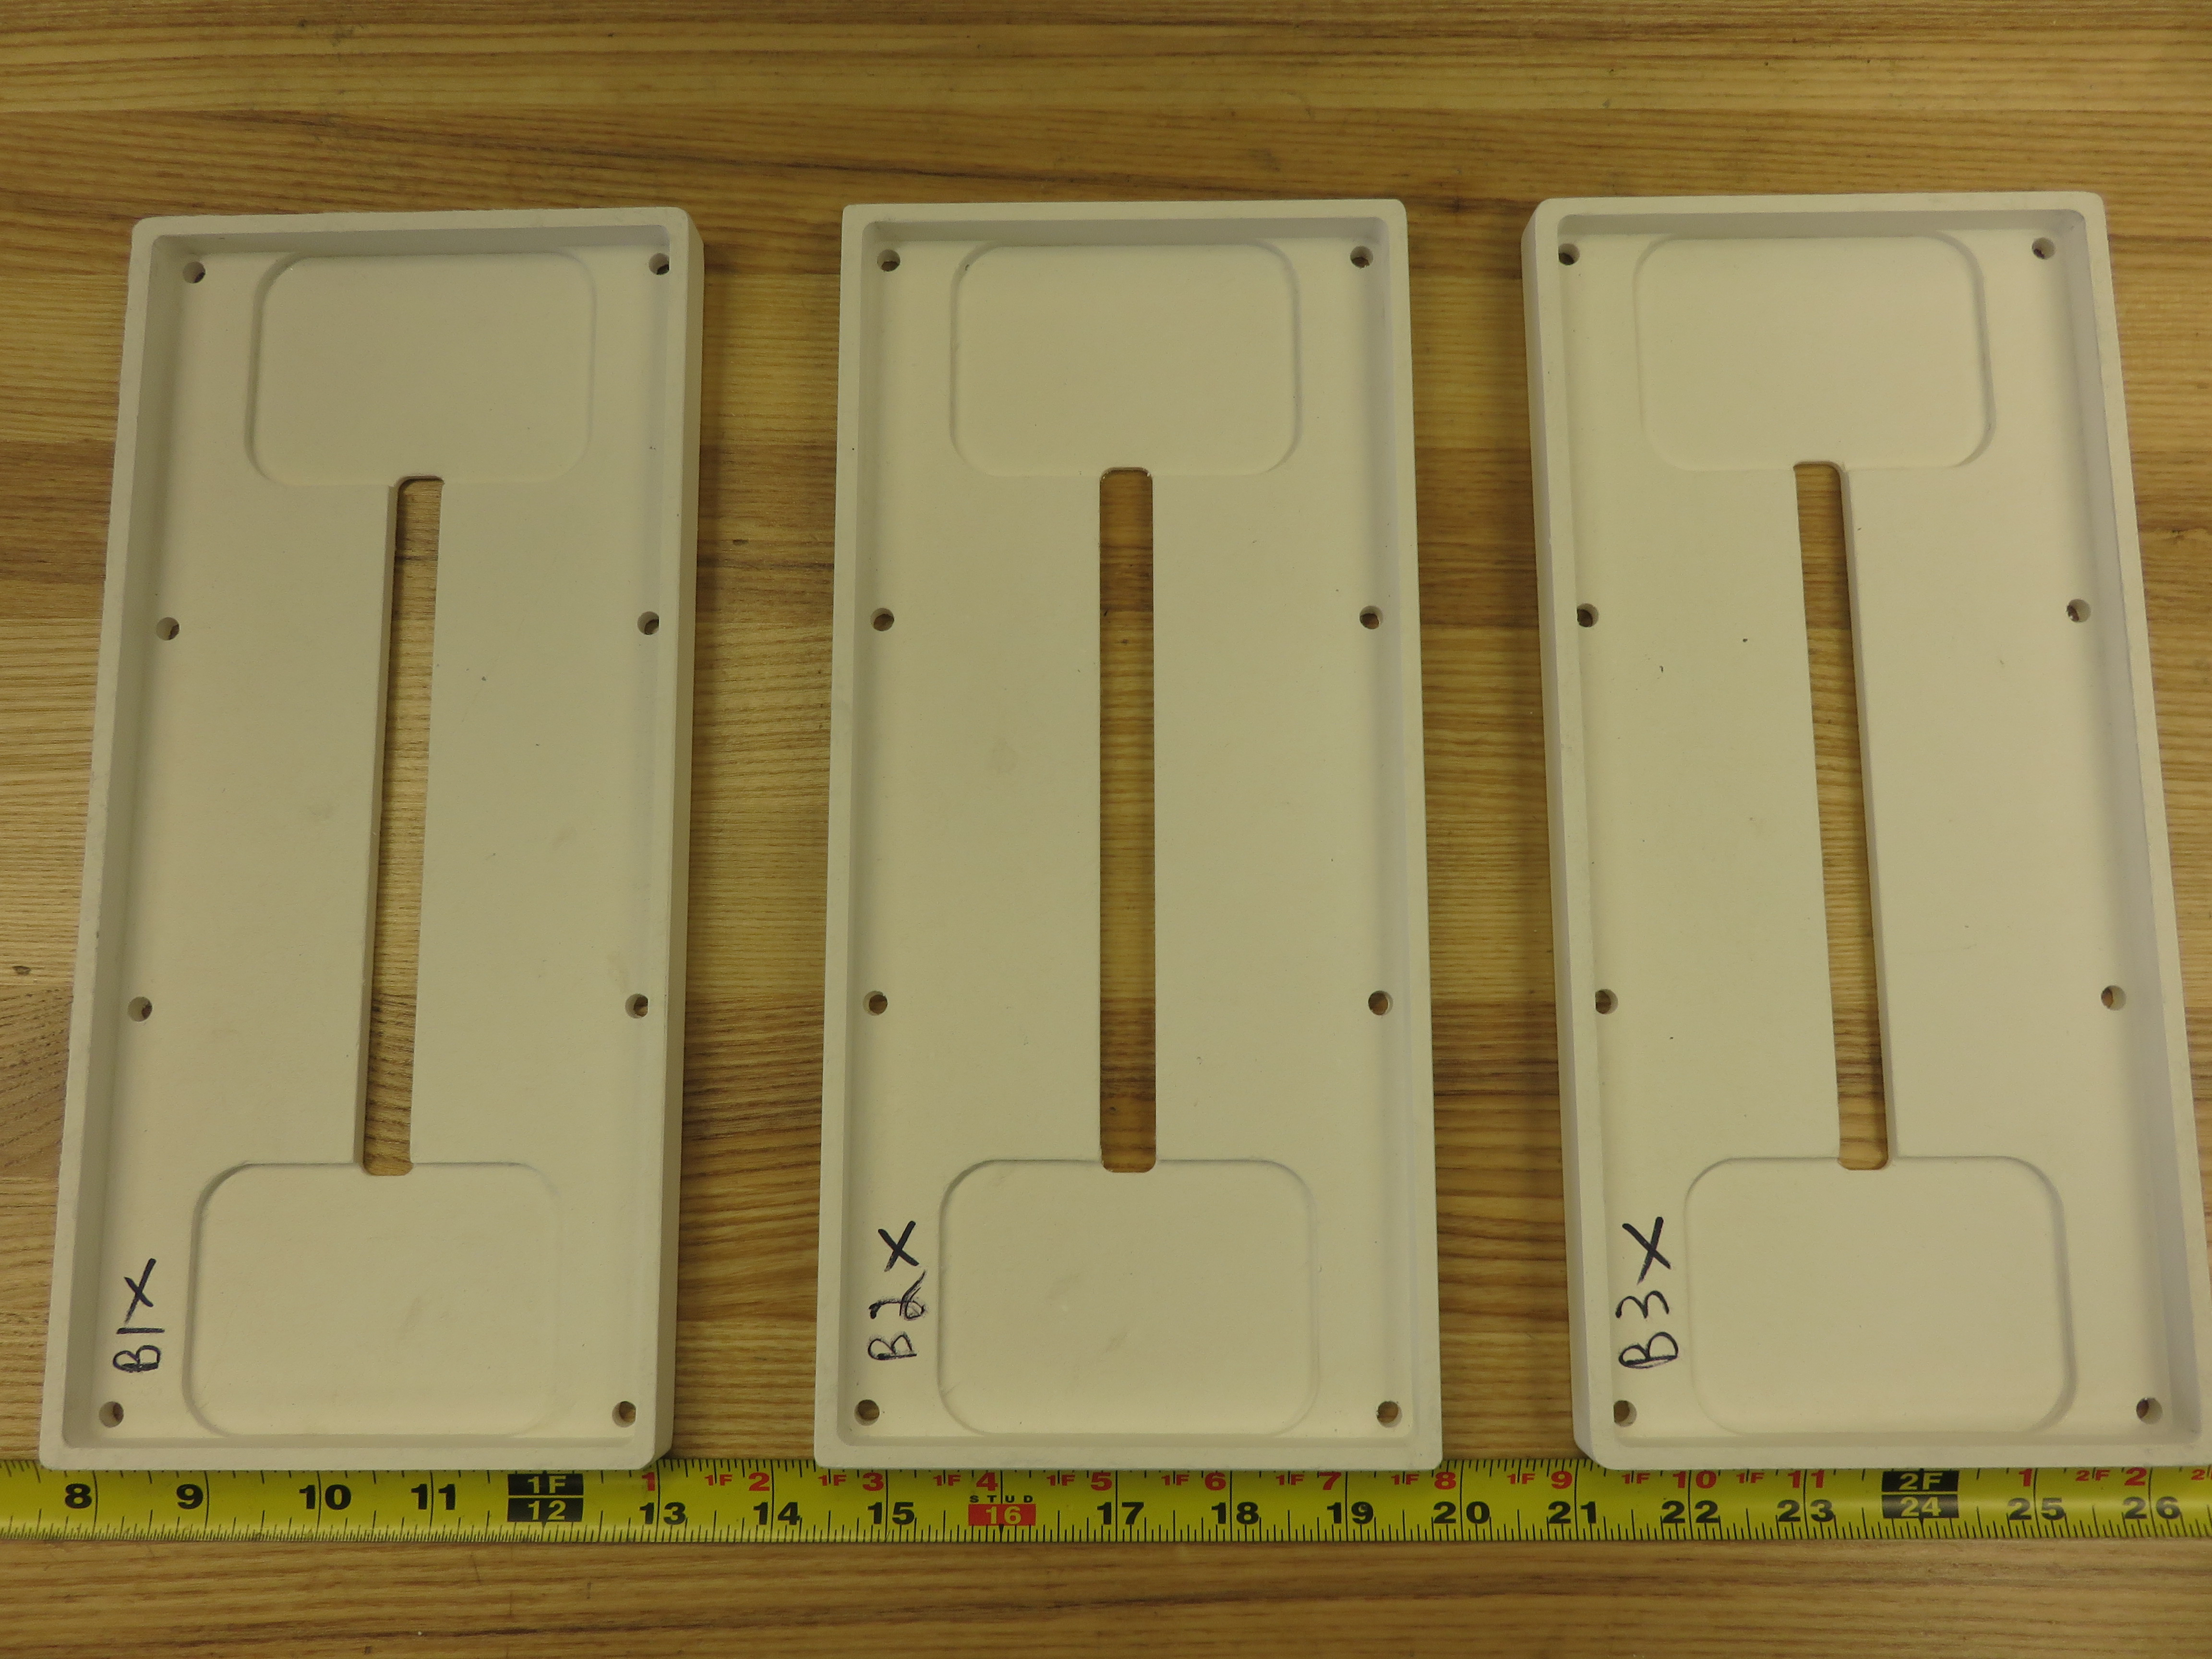
\includegraphics[scale=0.1]{facility/MachinedParts/B_insul_v2.JPG}}}
   {\subfigcapskip = 5pt \subfigcapmargin = -12pt  \subfigure[]{\label{fig:edge-b}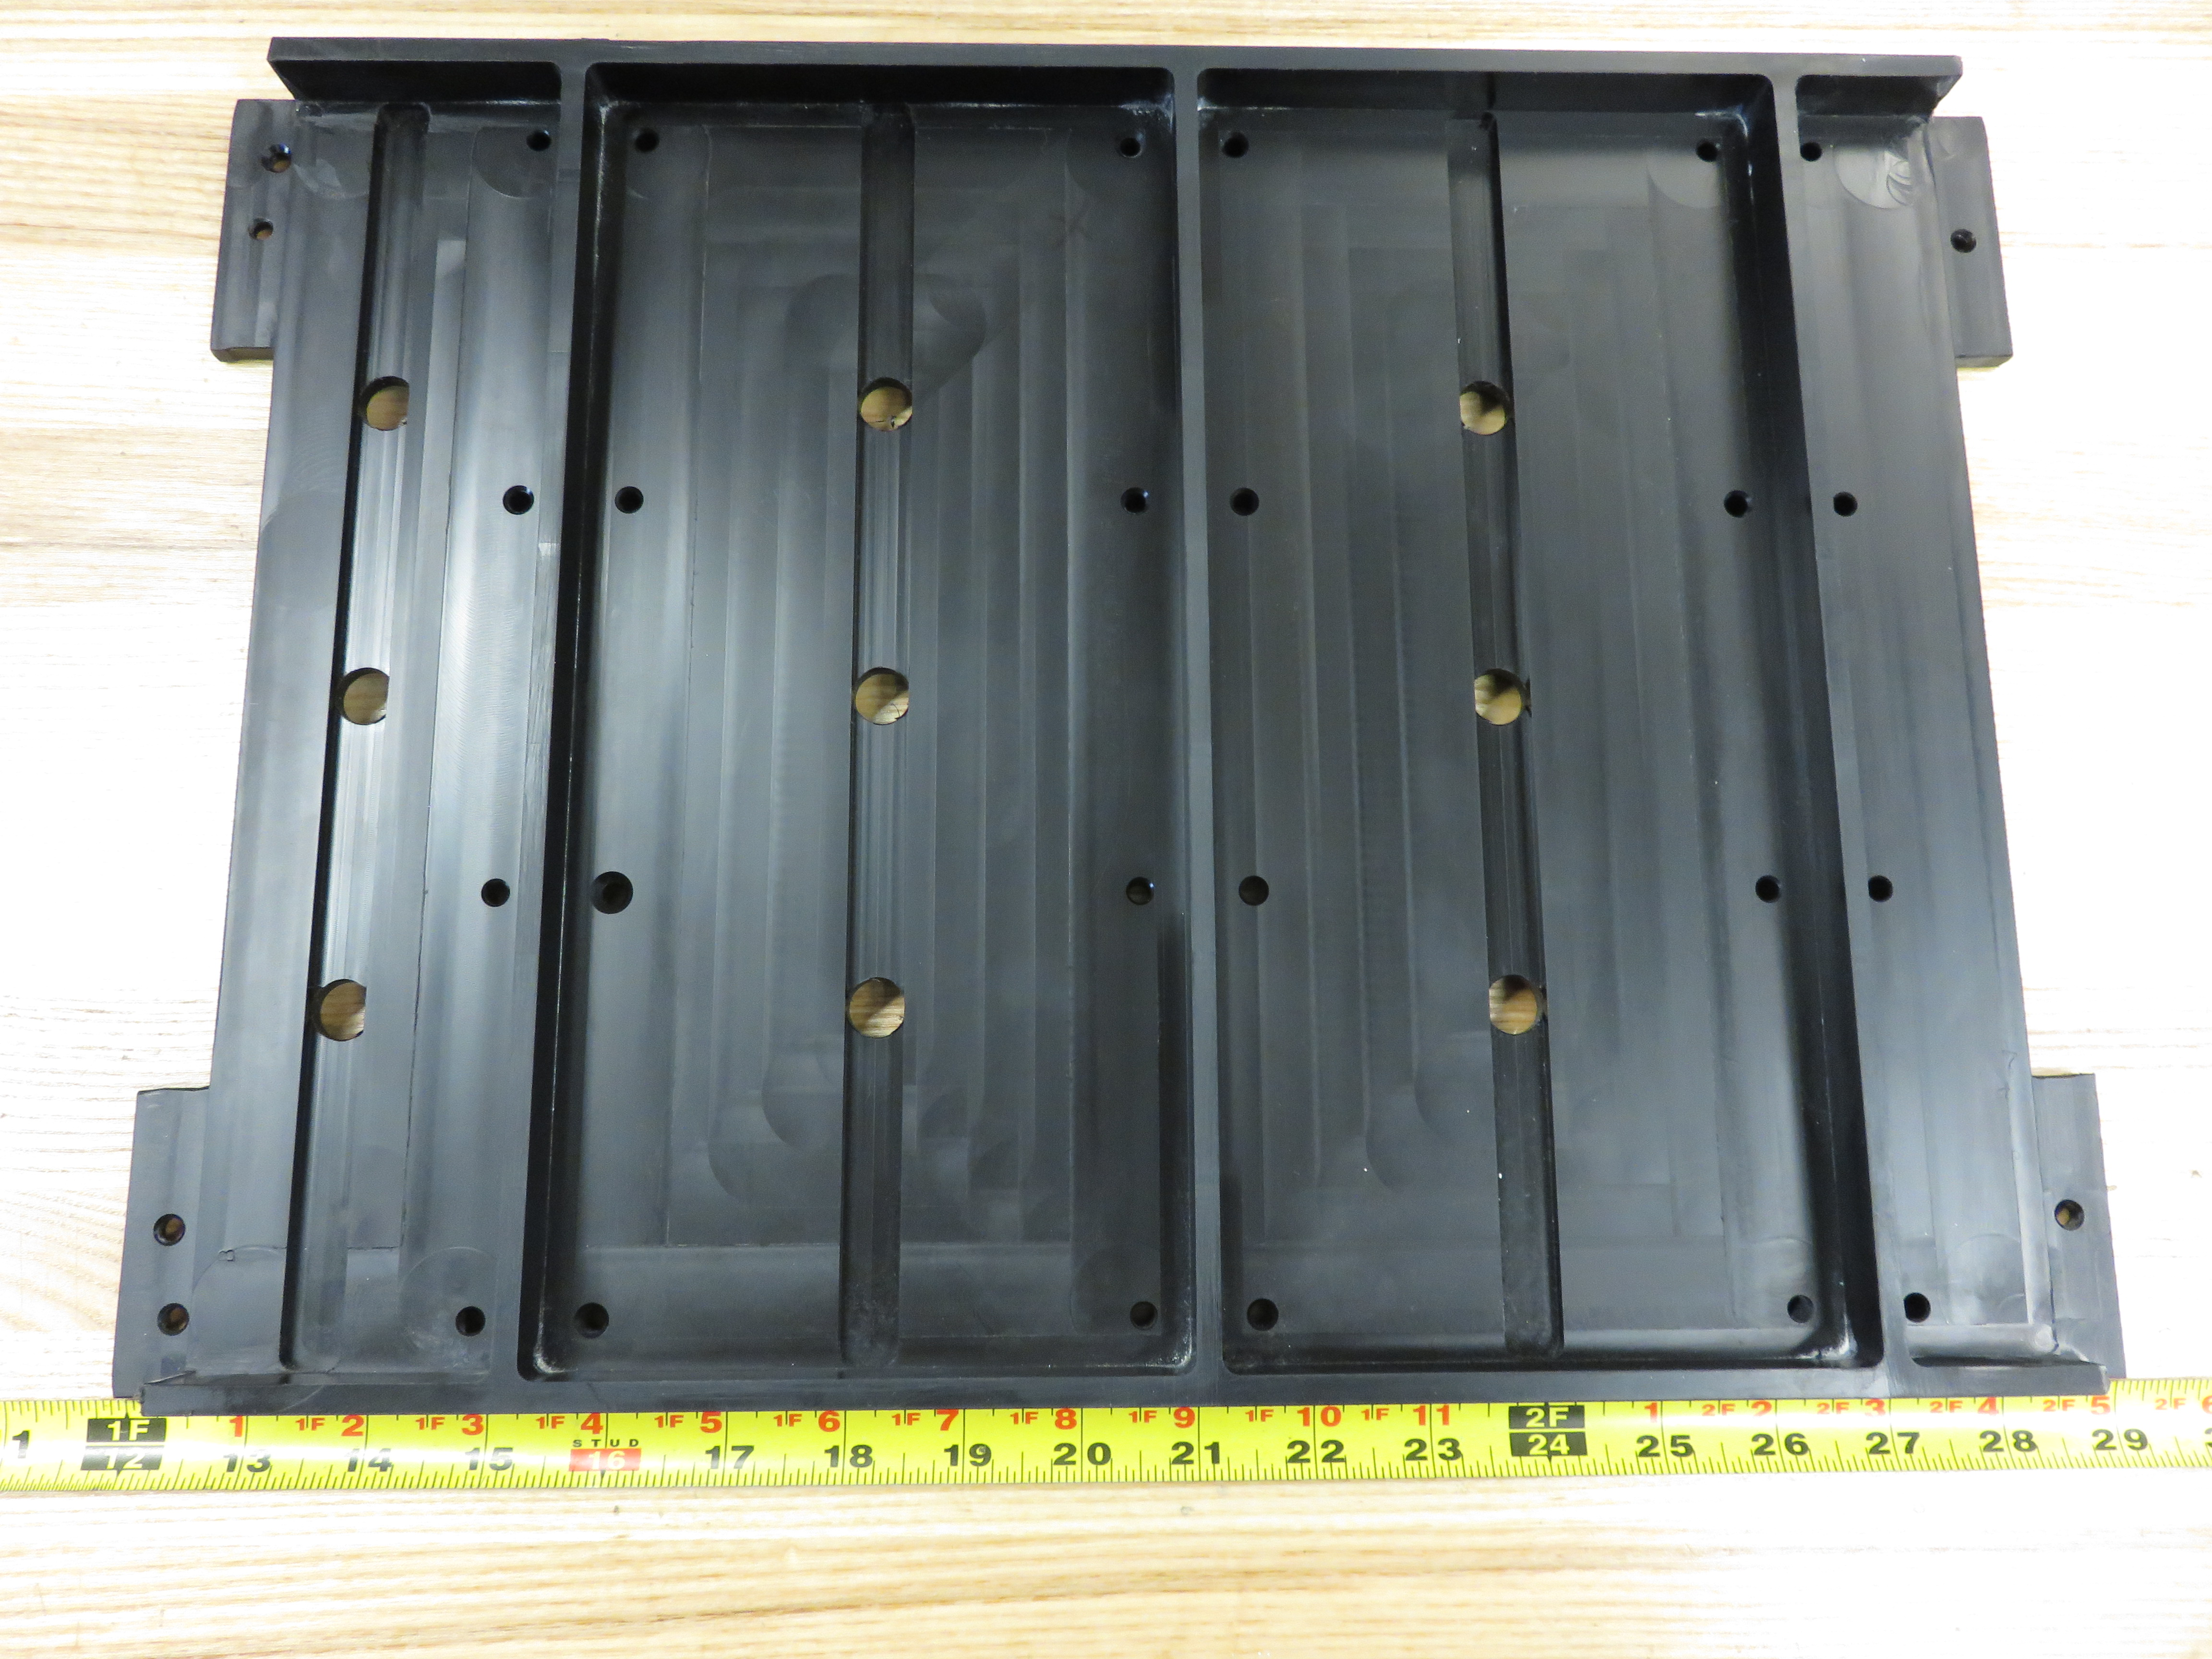
\includegraphics[scale=0.1]{facility/MachinedParts/B_meas_v2.JPG}}}
  \end{center}
\caption{(a) insulation (b) frame. } 
\label{fig:partsB}
\end{figure}

\begin{figure}[h!]
  \begin{center}
  {\subfigcapskip = 5pt \subfigcapmargin = -12pt \subfigure[]{\label{fig:edge-a}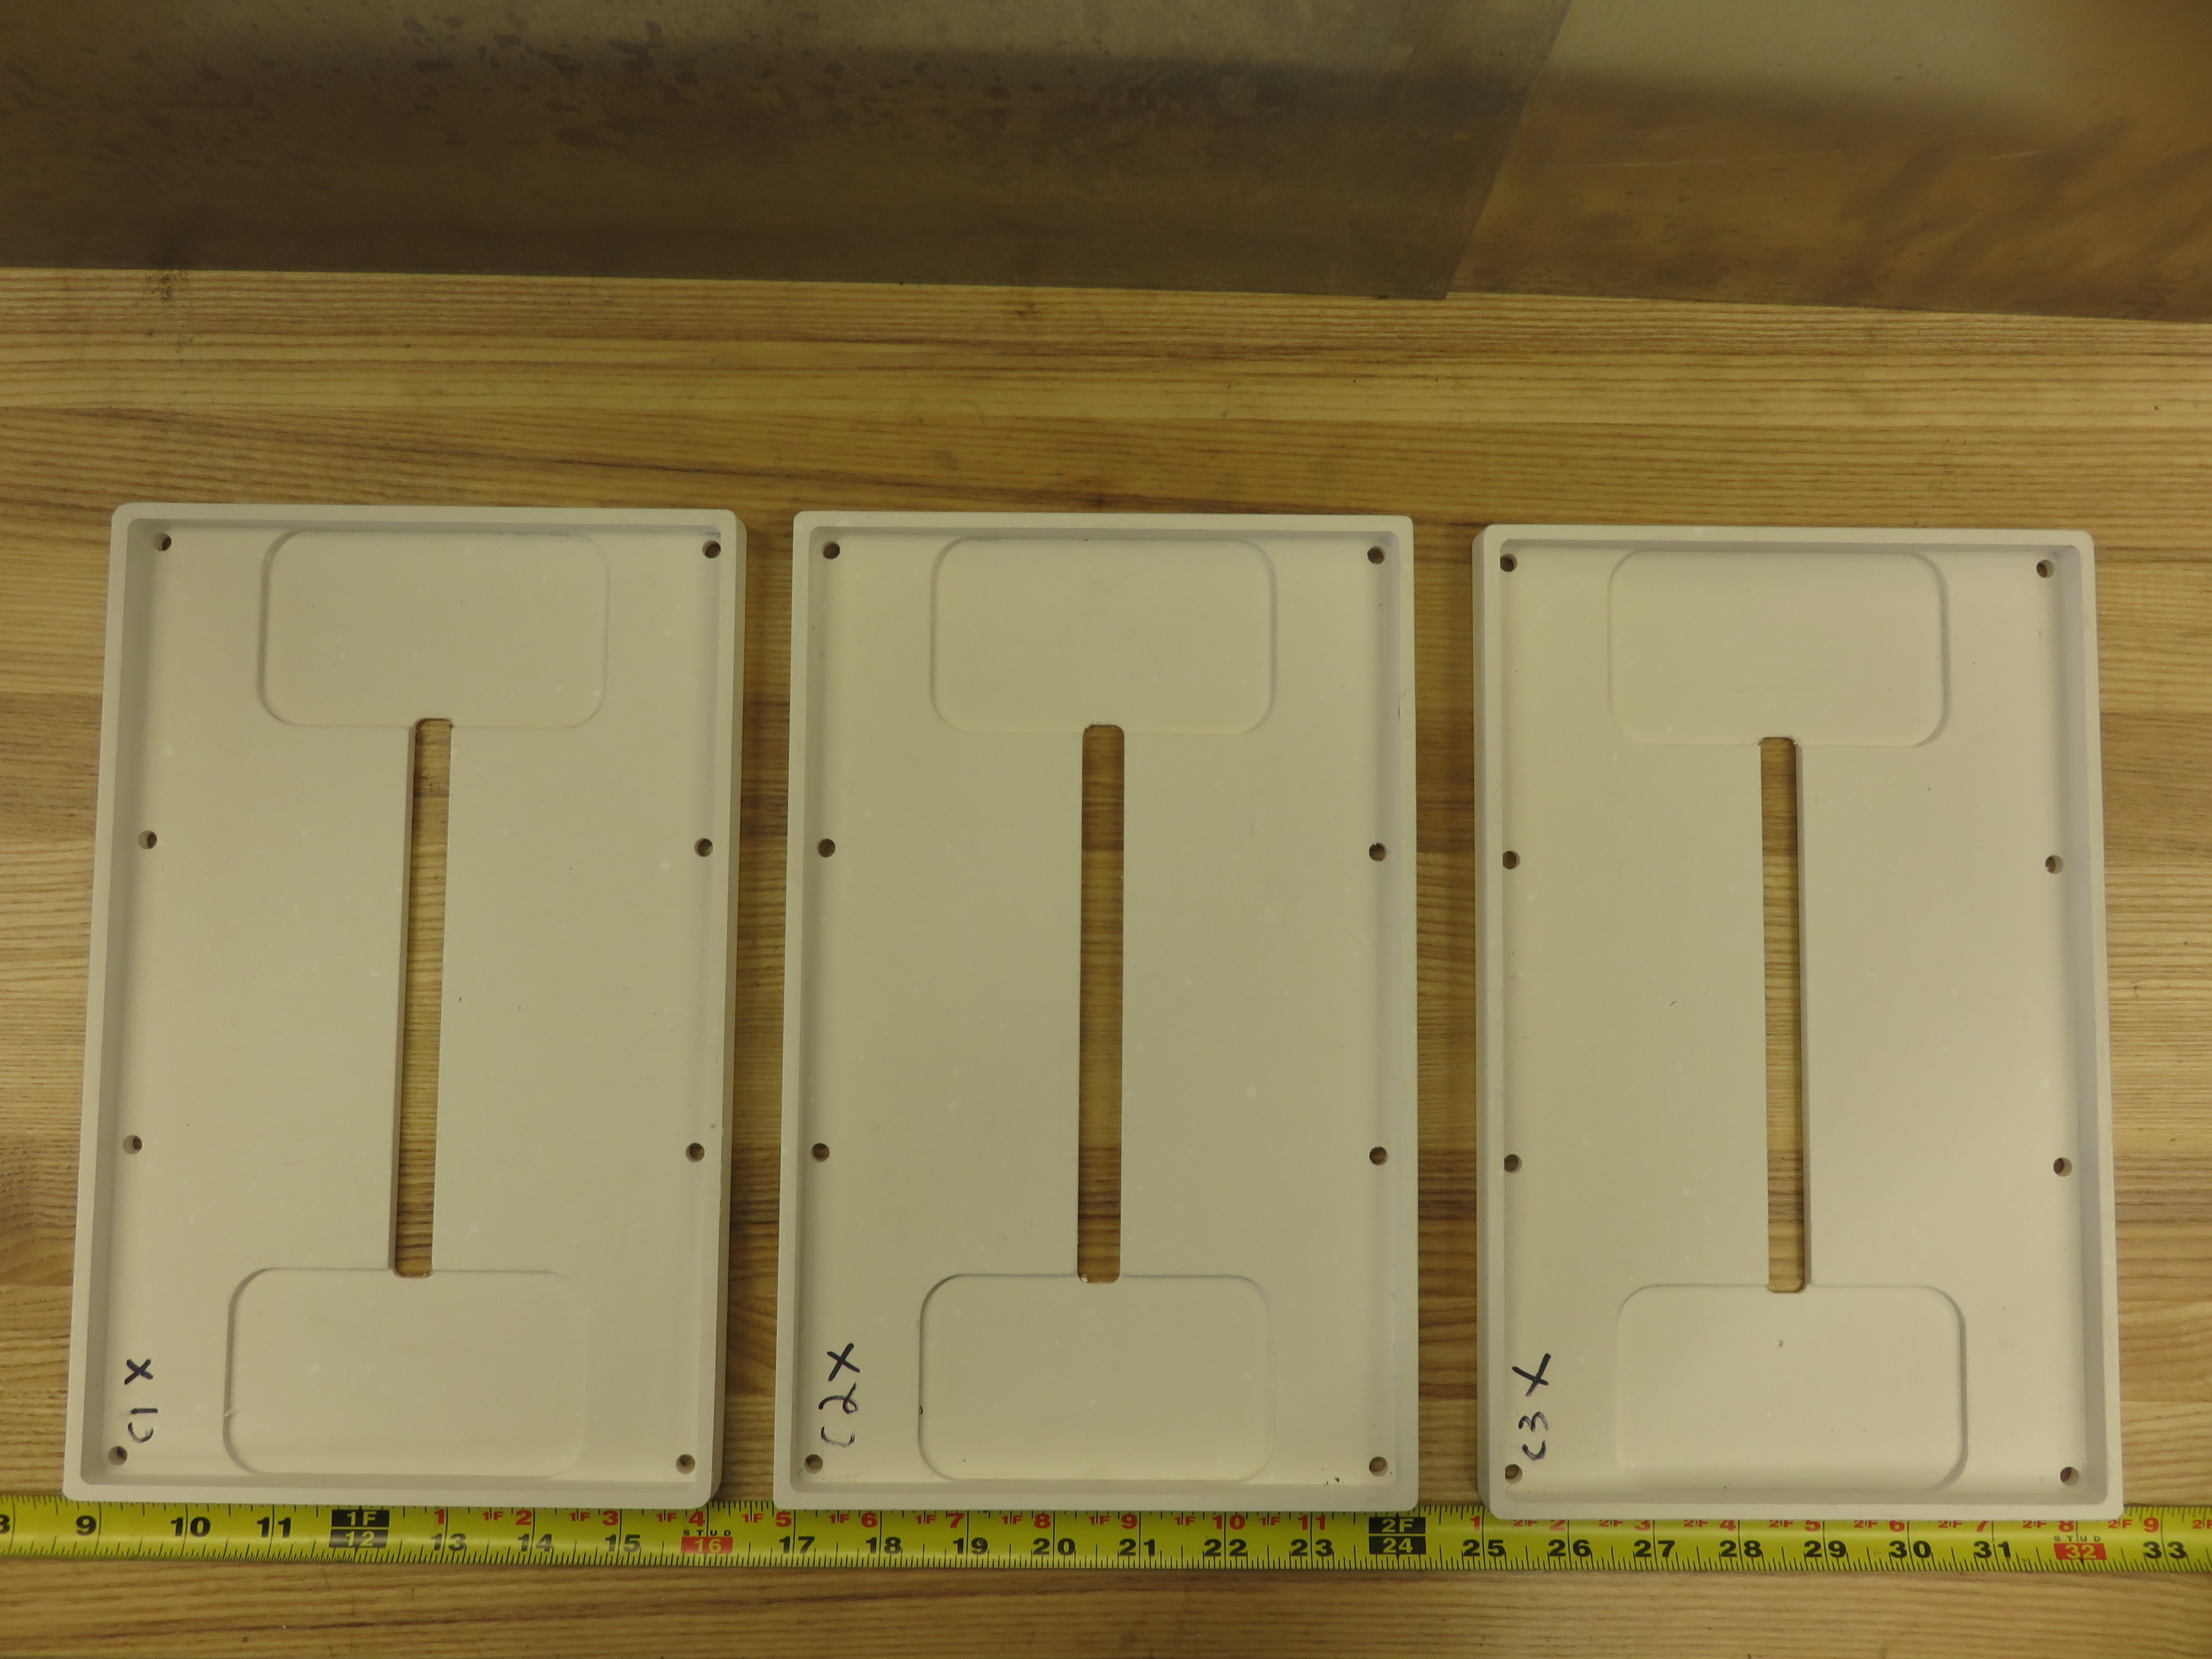
\includegraphics[scale=0.1]{facility/MachinedParts/C_insul_v1.JPG}}}
   {\subfigcapskip = 5pt \subfigcapmargin = -12pt  \subfigure[]{\label{fig:edge-b}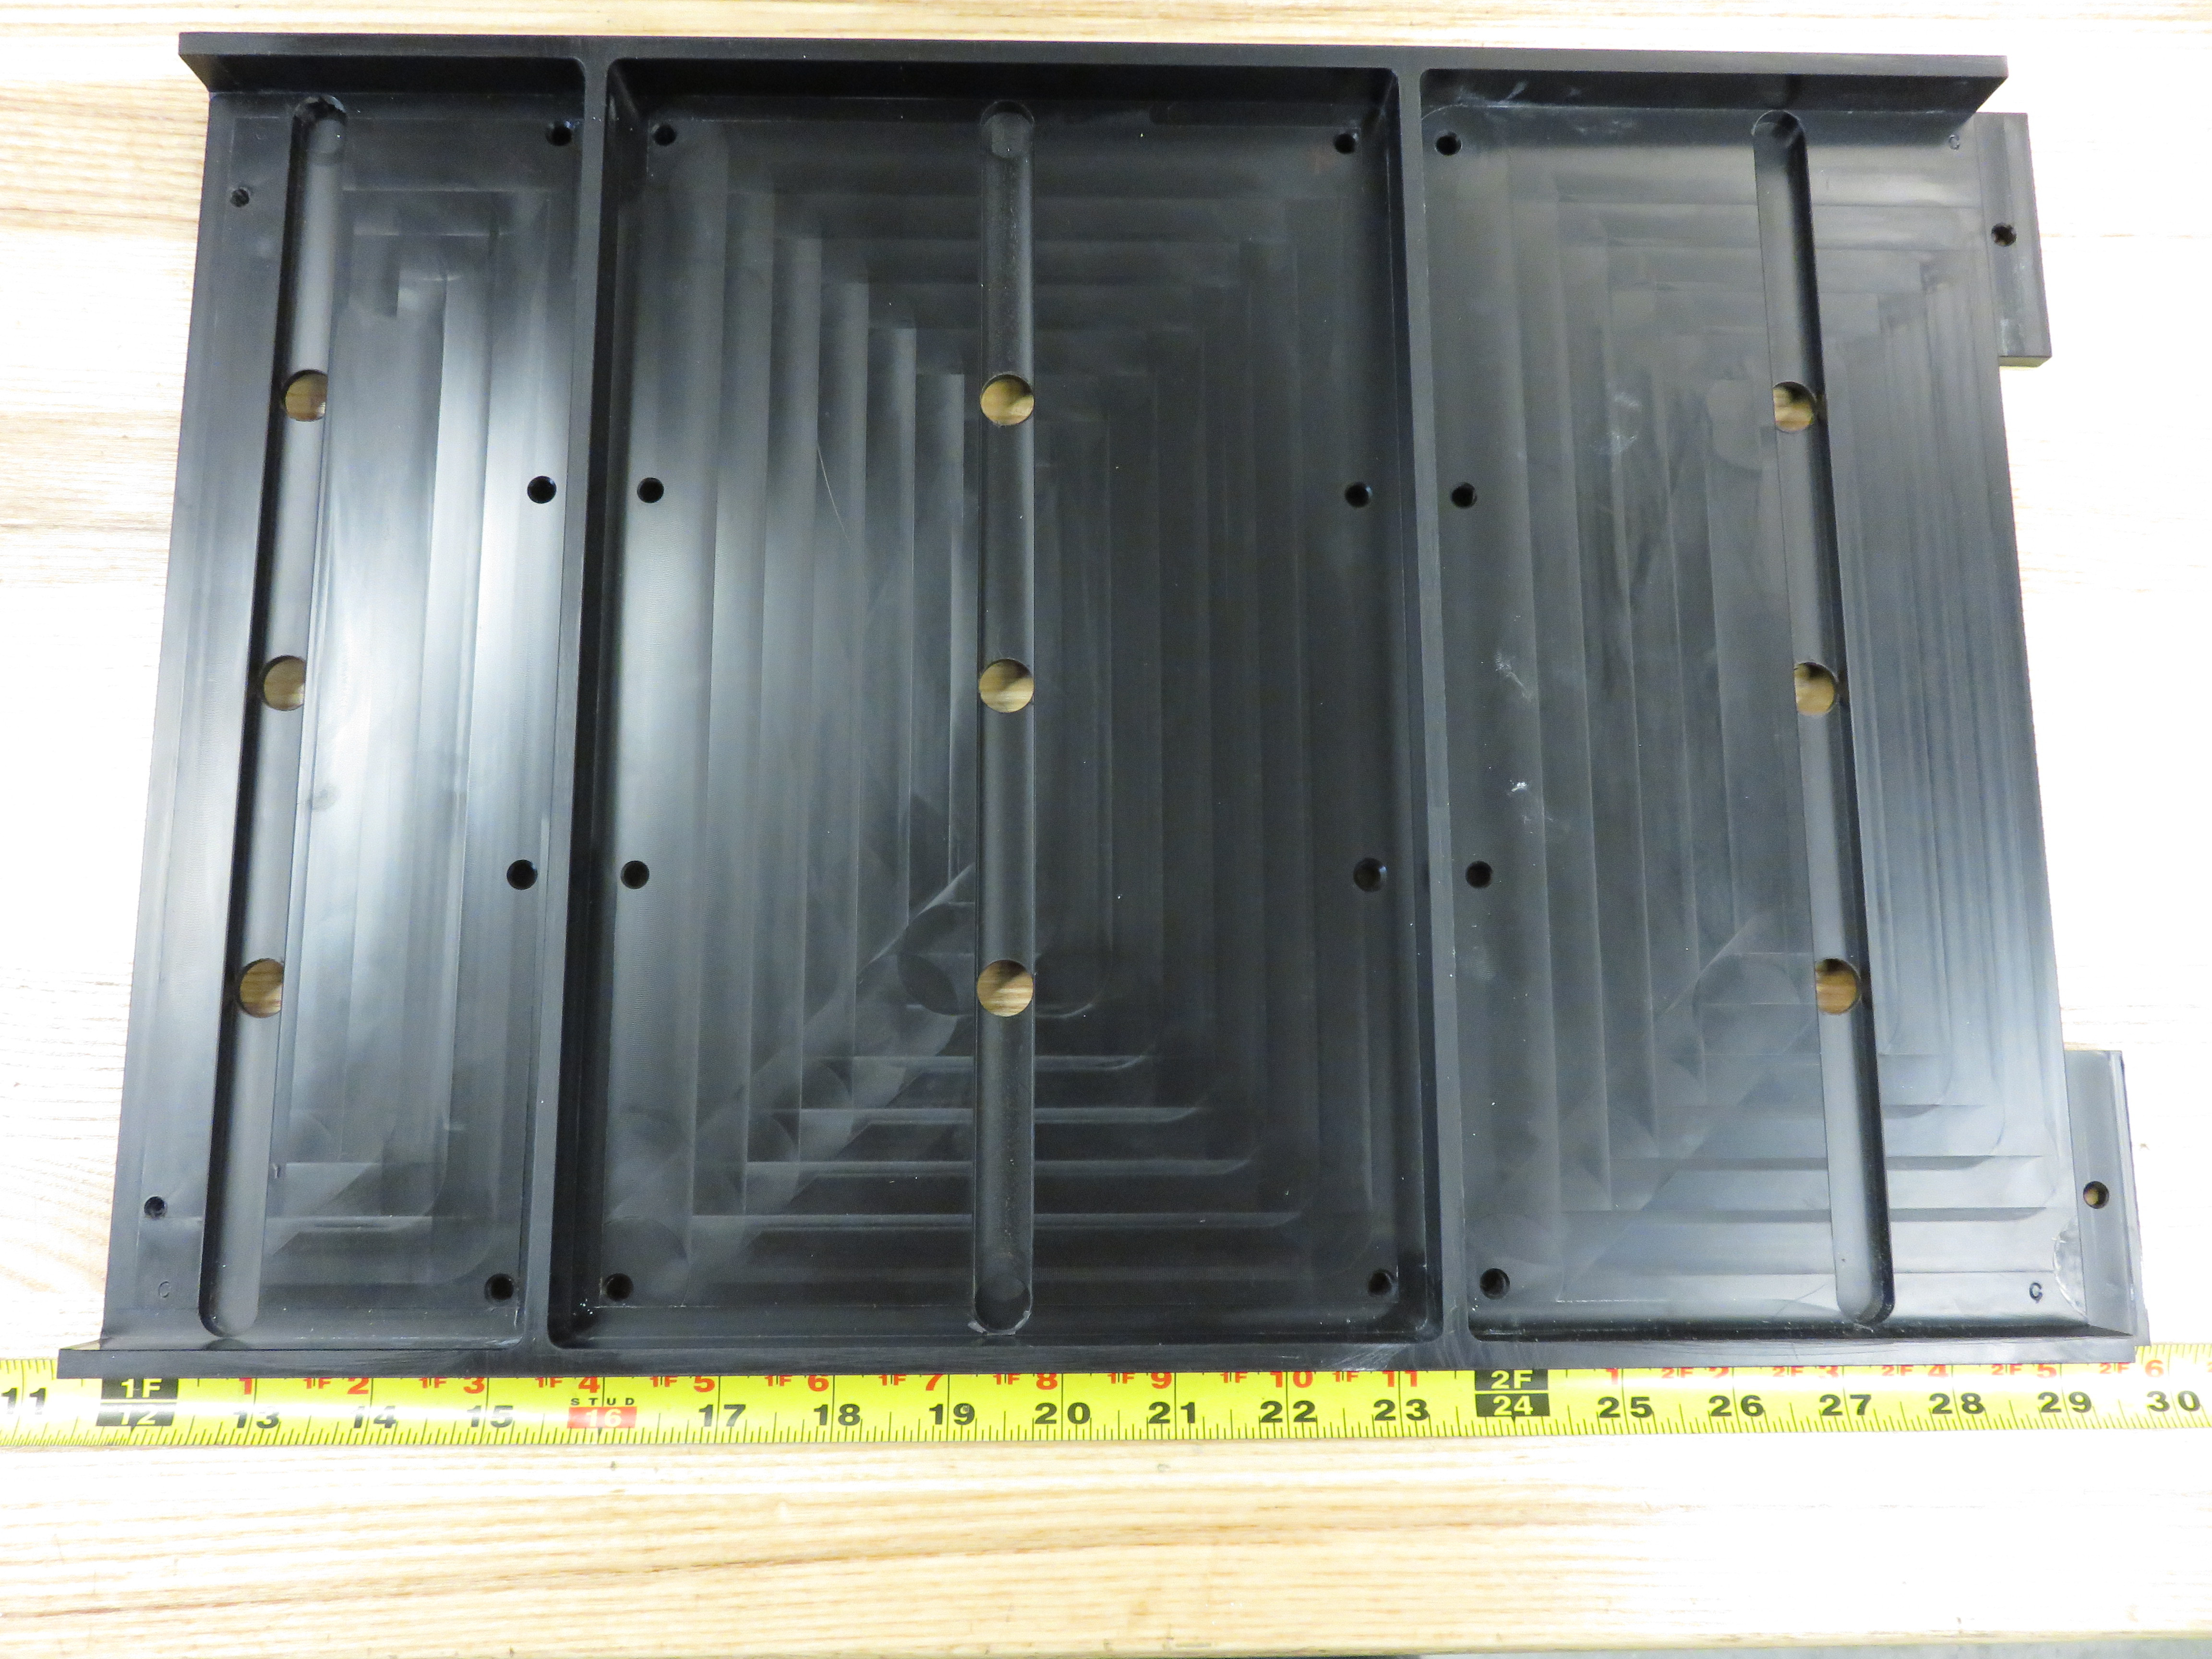
\includegraphics[scale=0.1]{facility/MachinedParts/C_meas_v2.JPG}}}
  \end{center}
\caption{(a) insulation (b) frame. } 
\label{fig:partsC}
\end{figure}

\begin{figure}[h!]
  \begin{center}
  {\subfigcapskip = 5pt \subfigcapmargin = -12pt \subfigure[]{\label{fig:edge-a}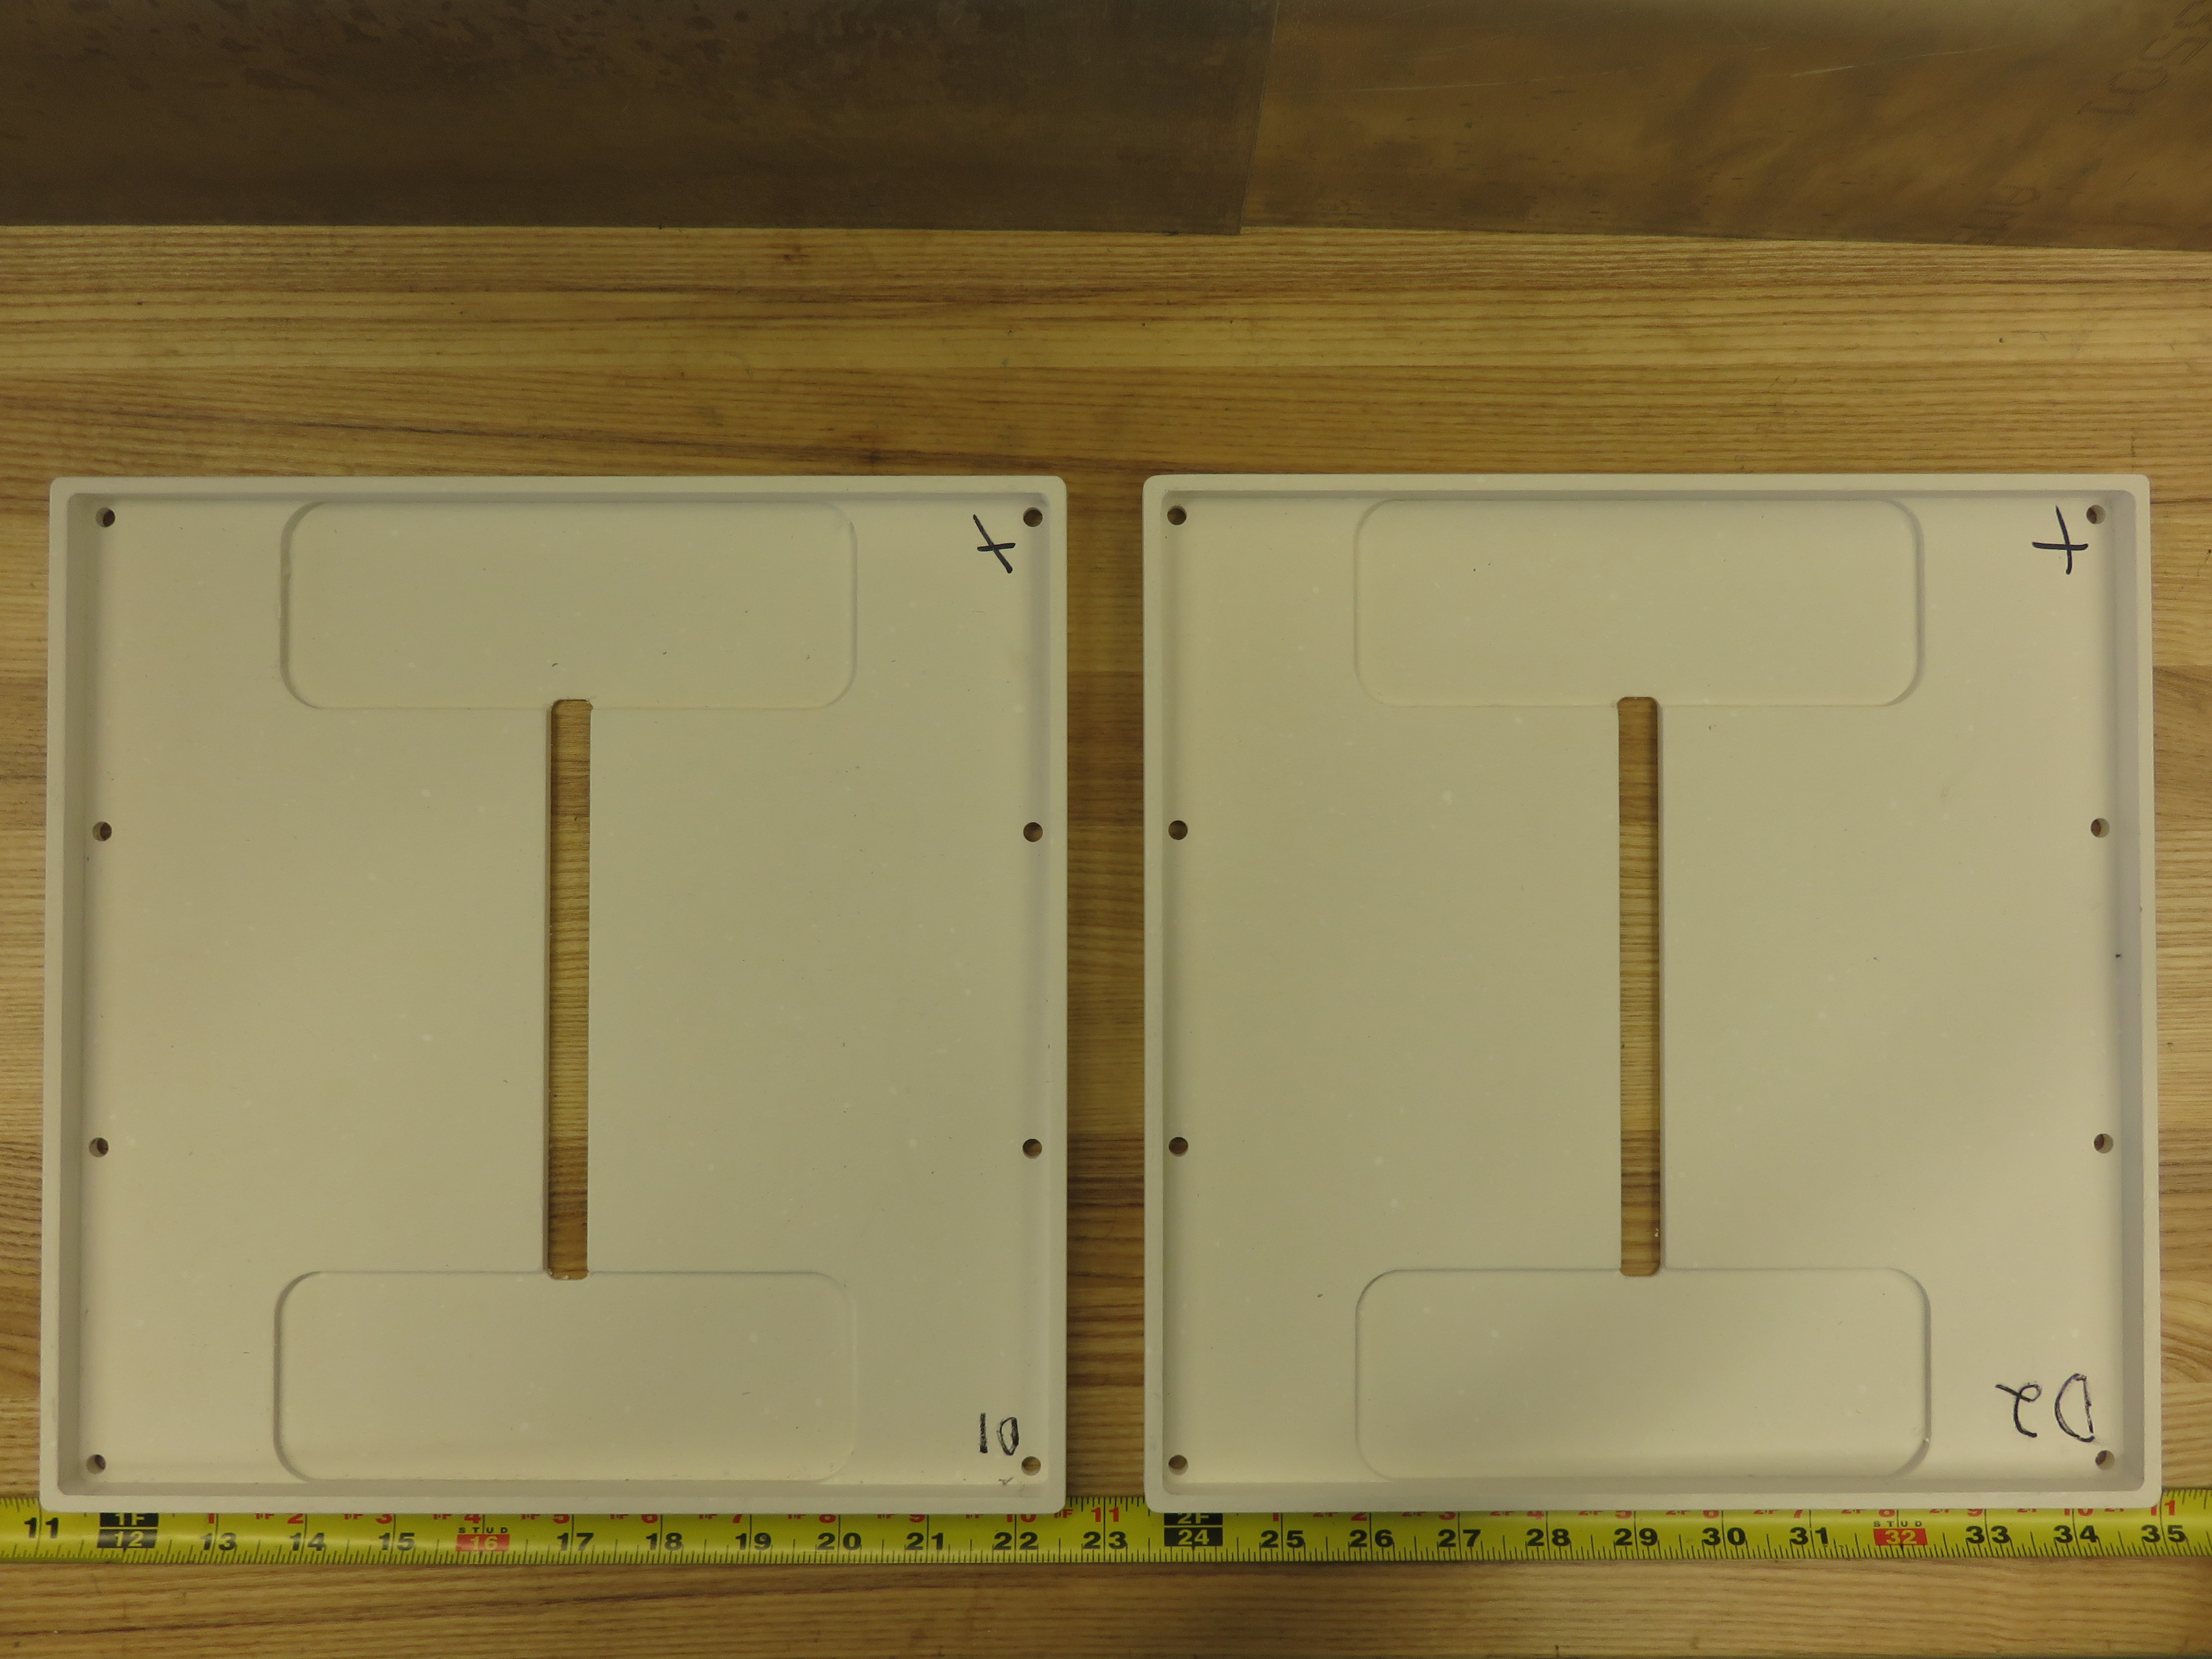
\includegraphics[scale=0.1]{facility/MachinedParts/D_insul_v2.JPG}}}
   {\subfigcapskip = 5pt \subfigcapmargin = -12pt  \subfigure[]{\label{fig:edge-b}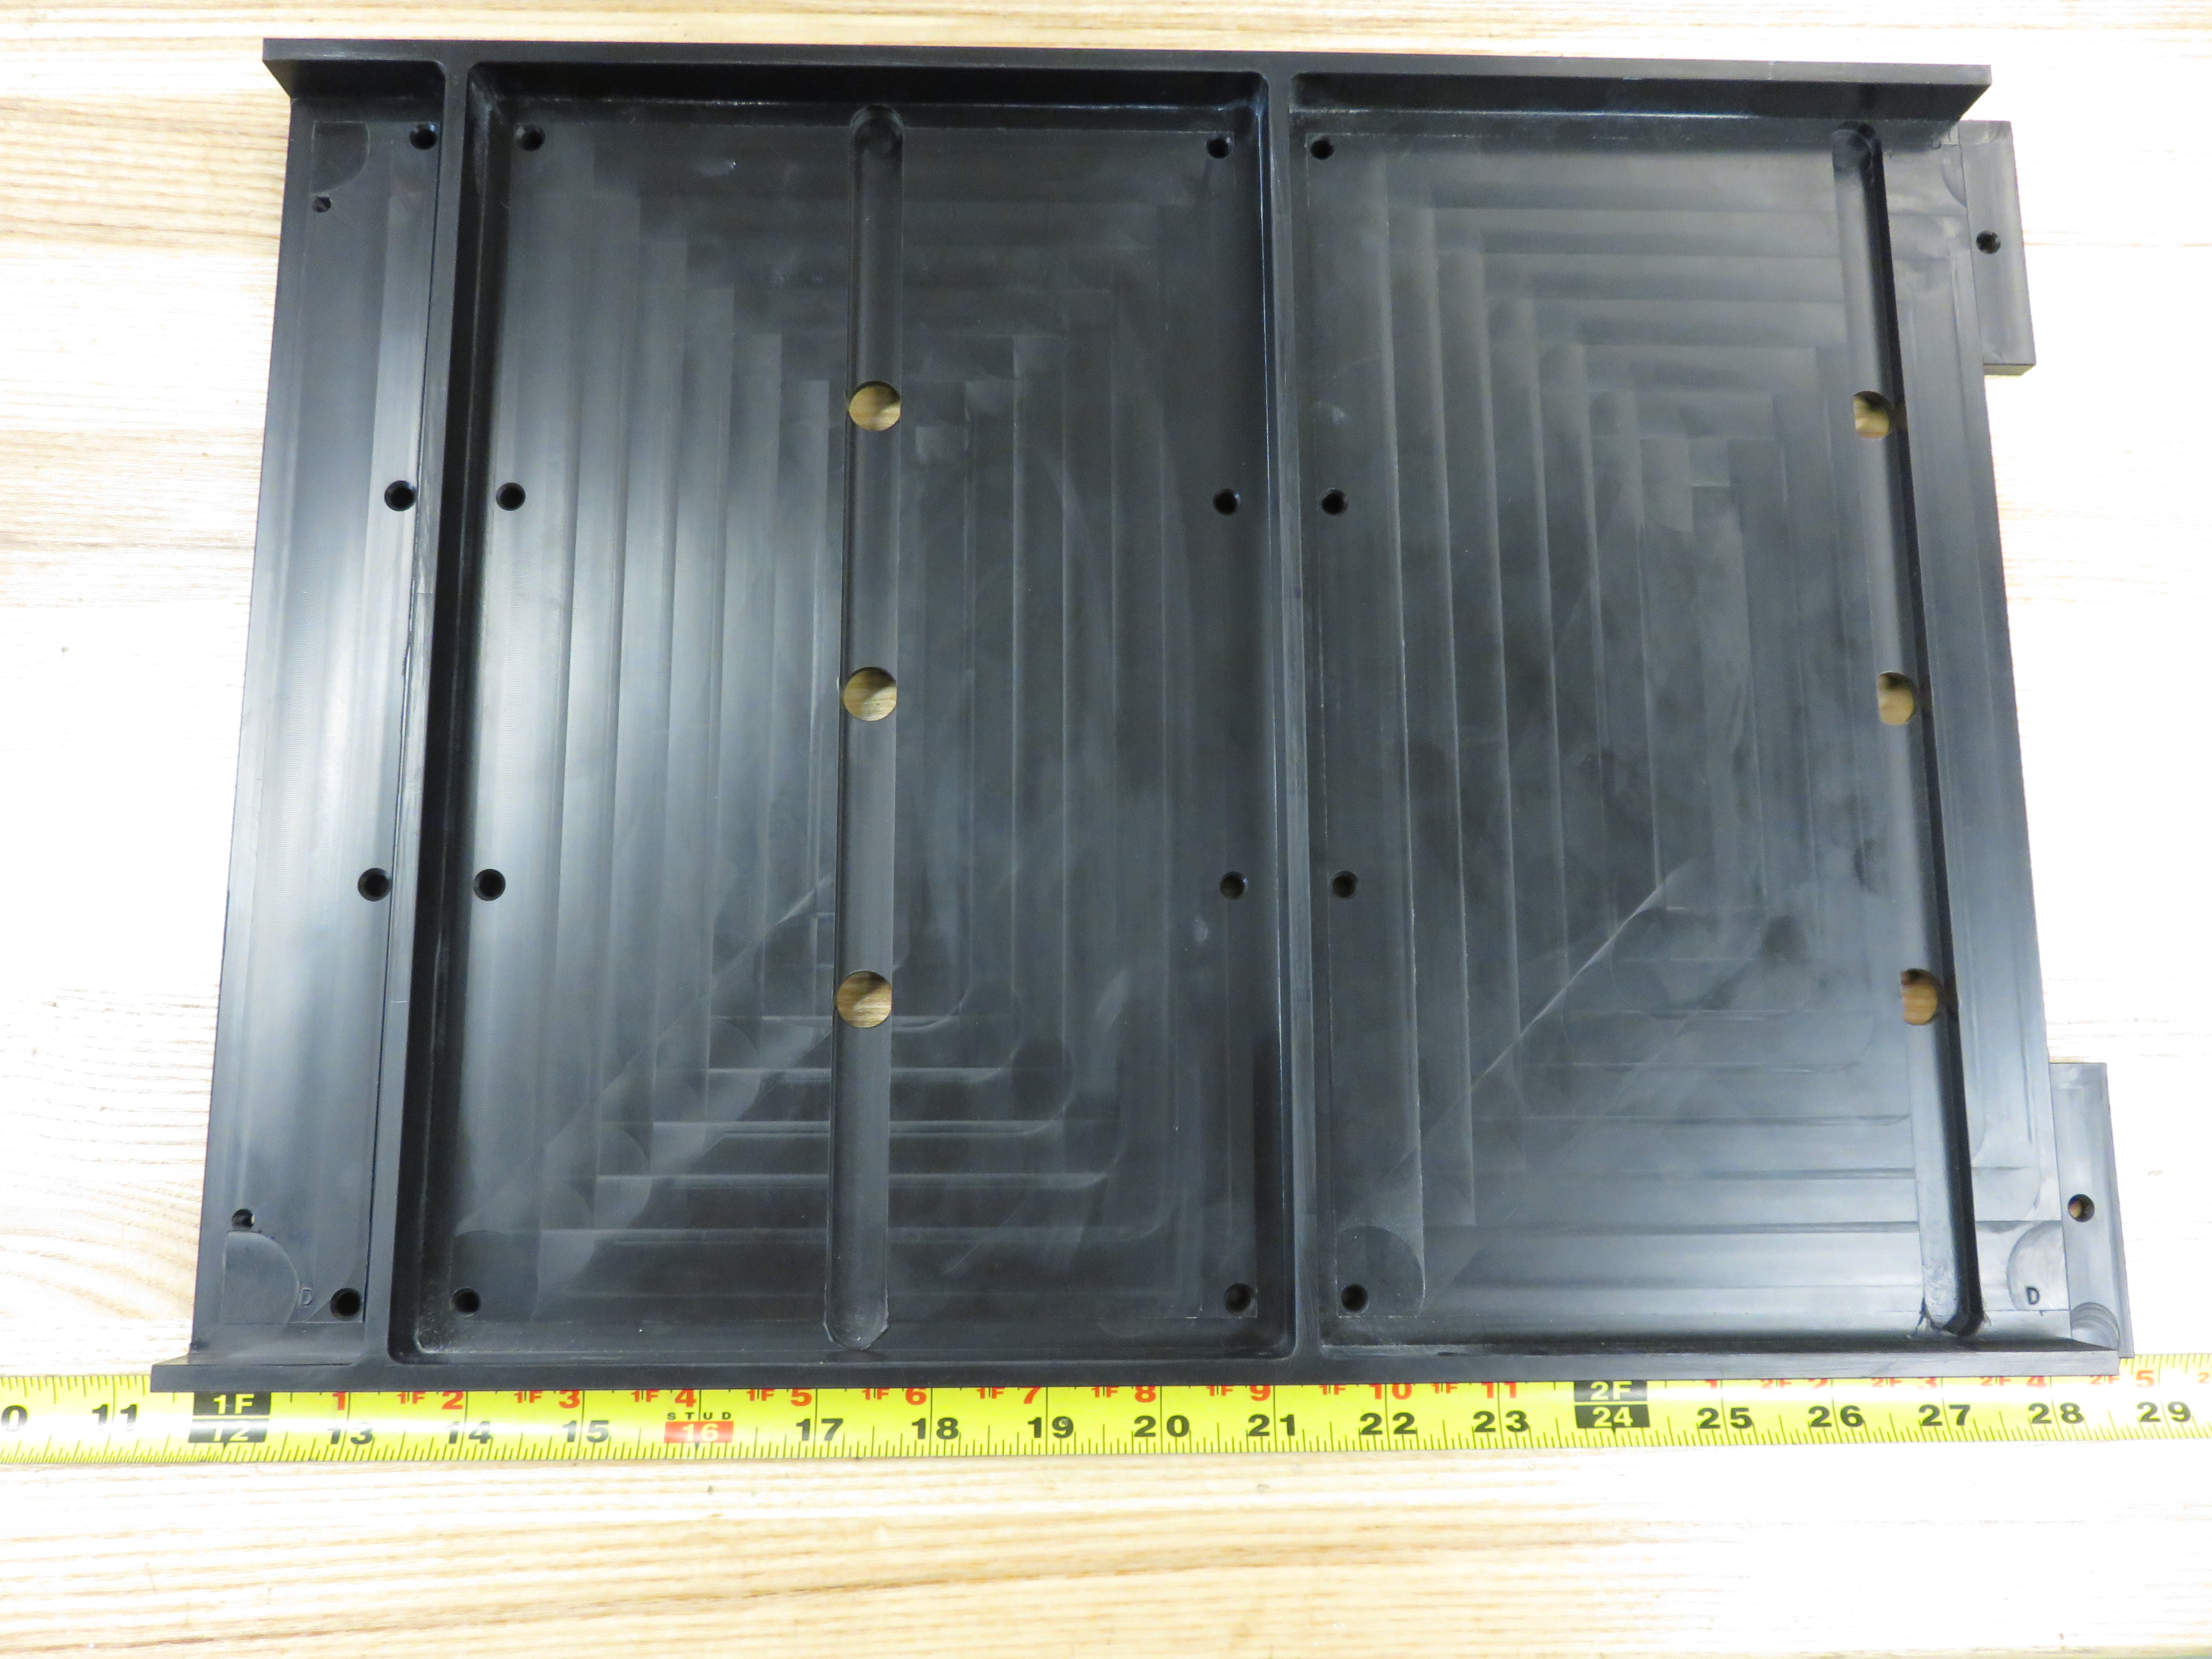
\includegraphics[scale=0.1]{facility/MachinedParts/D_meas_v2.JPG}}}
  \end{center}
\caption{(a) insulation (b) frame. } 
\label{fig:partsD}
\end{figure}

\begin{figure}[h!]
  \begin{center}
  {\subfigcapskip = 5pt \subfigcapmargin = -12pt \subfigure[]{\label{fig:edge-a}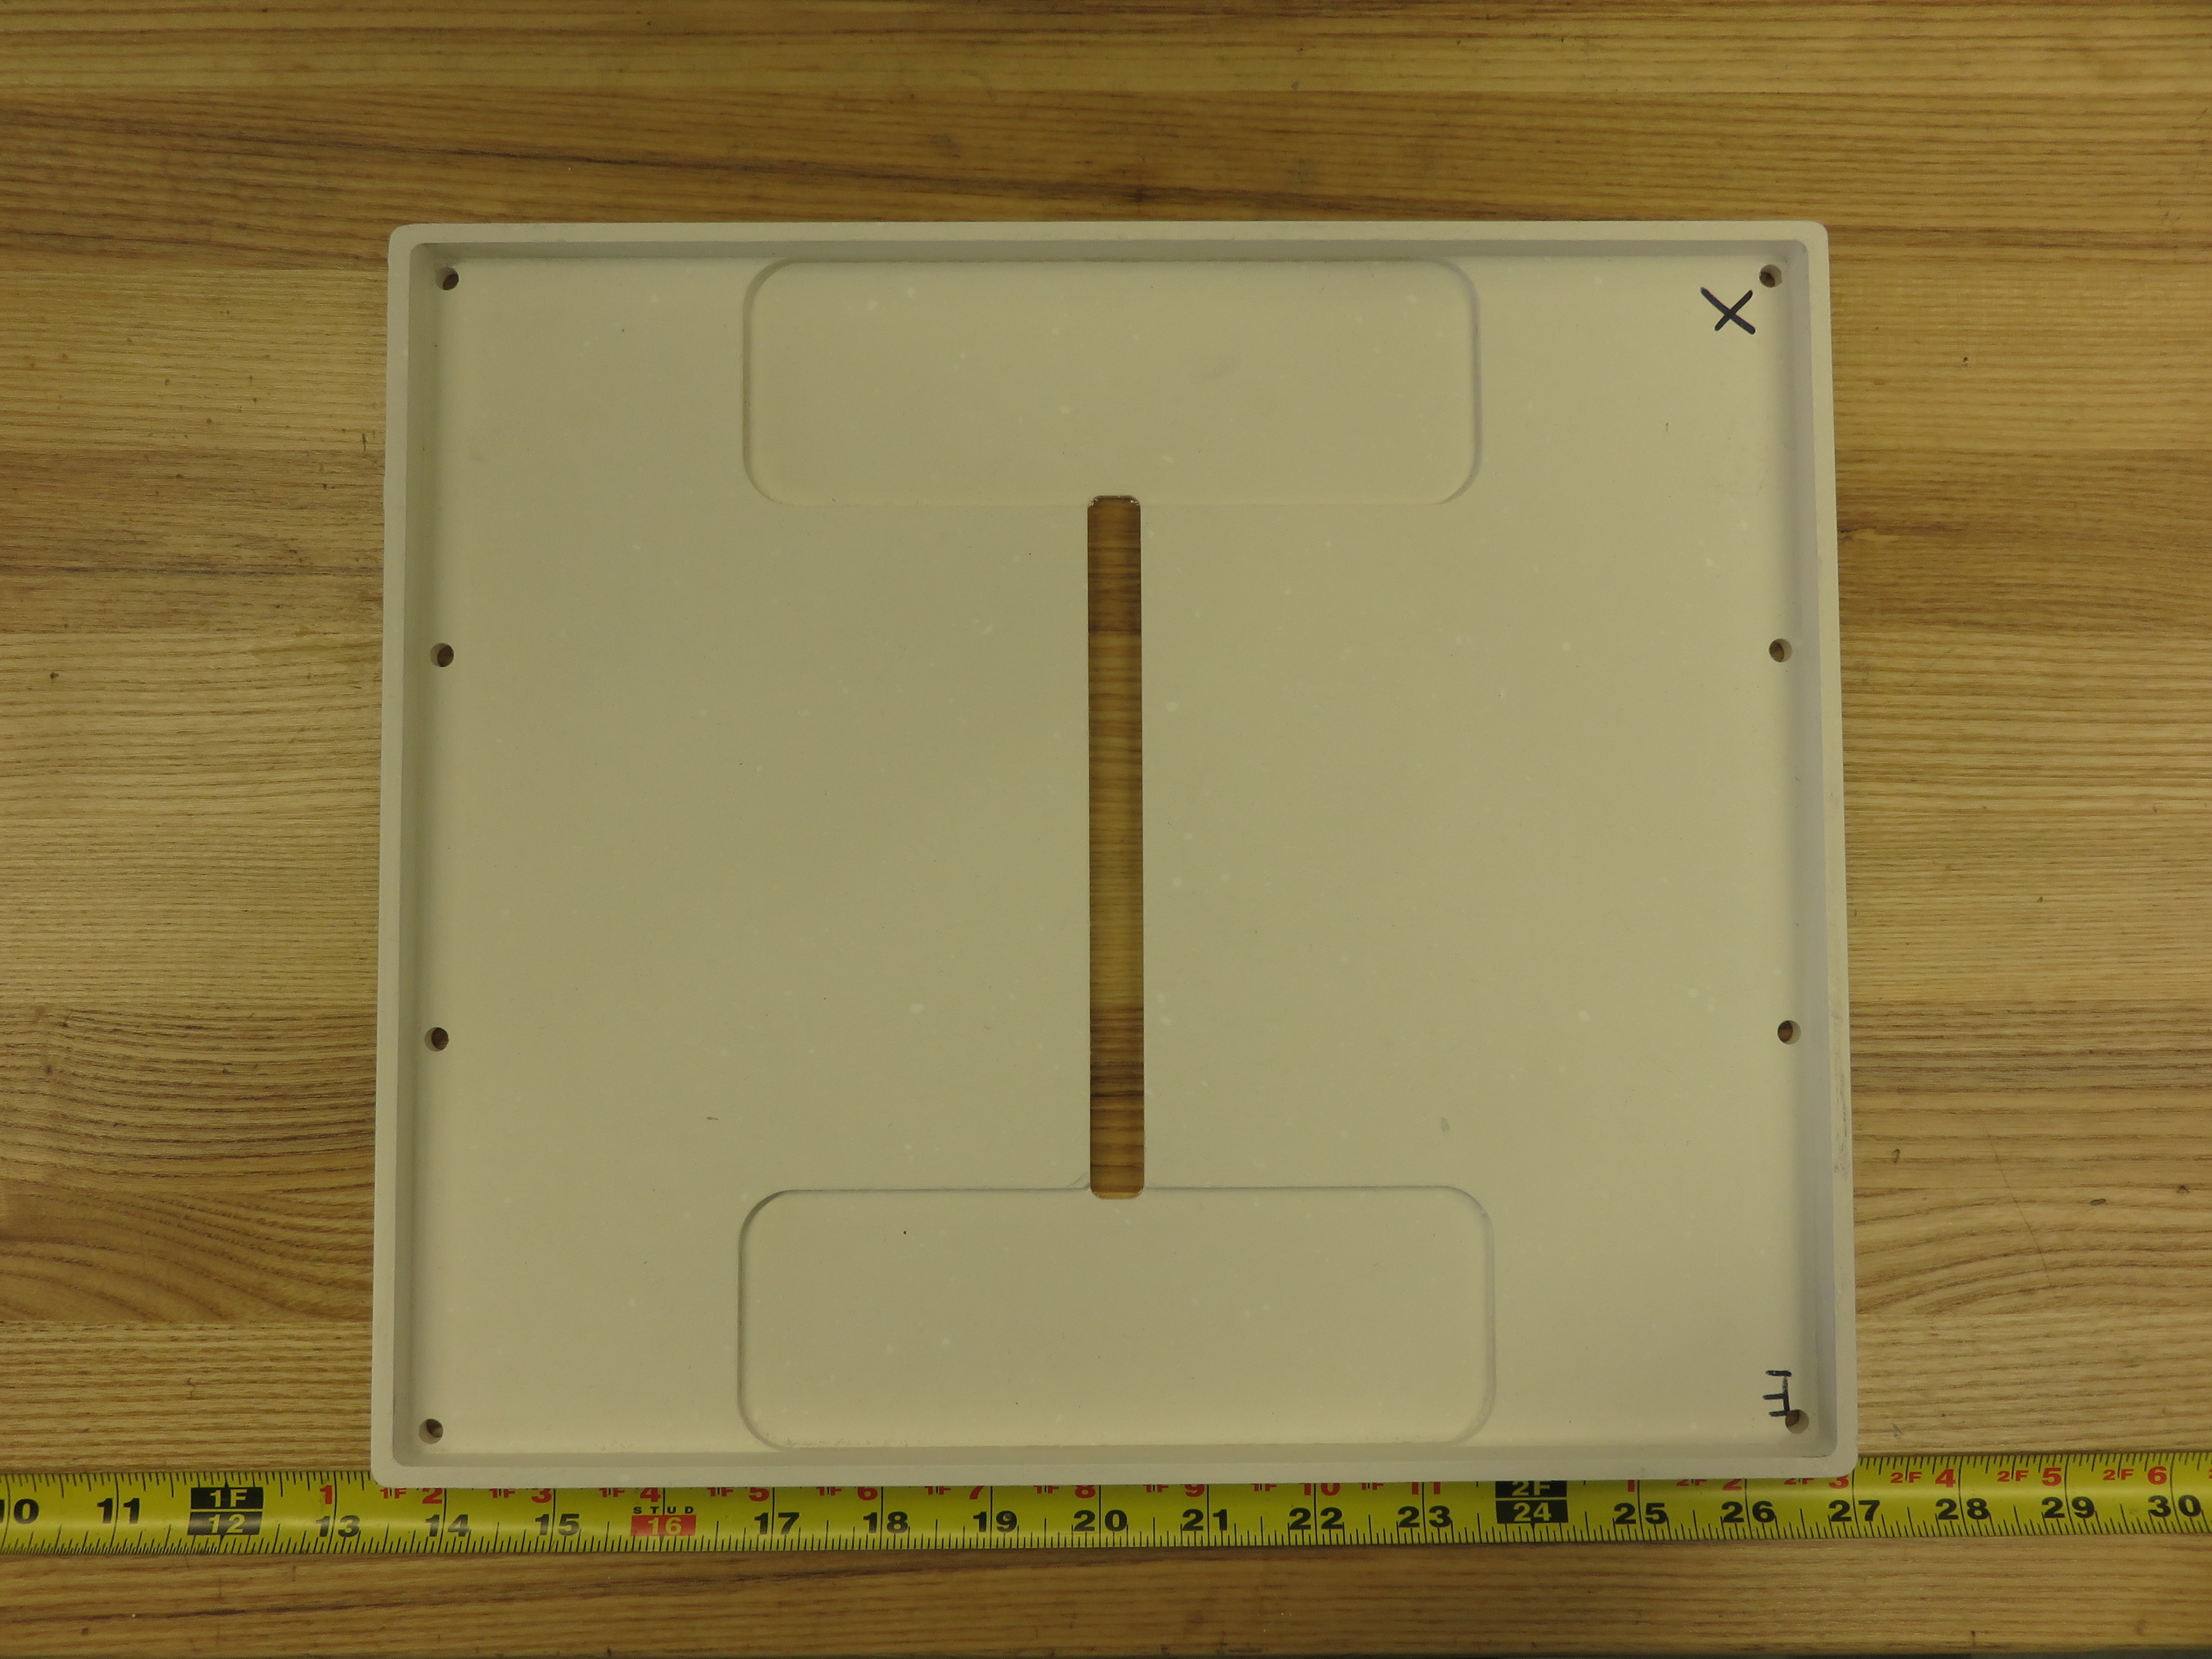
\includegraphics[scale=0.1]{facility/MachinedParts/E_insul_v2.JPG}}}
   {\subfigcapskip = 5pt \subfigcapmargin = -12pt  \subfigure[]{\label{fig:edge-b}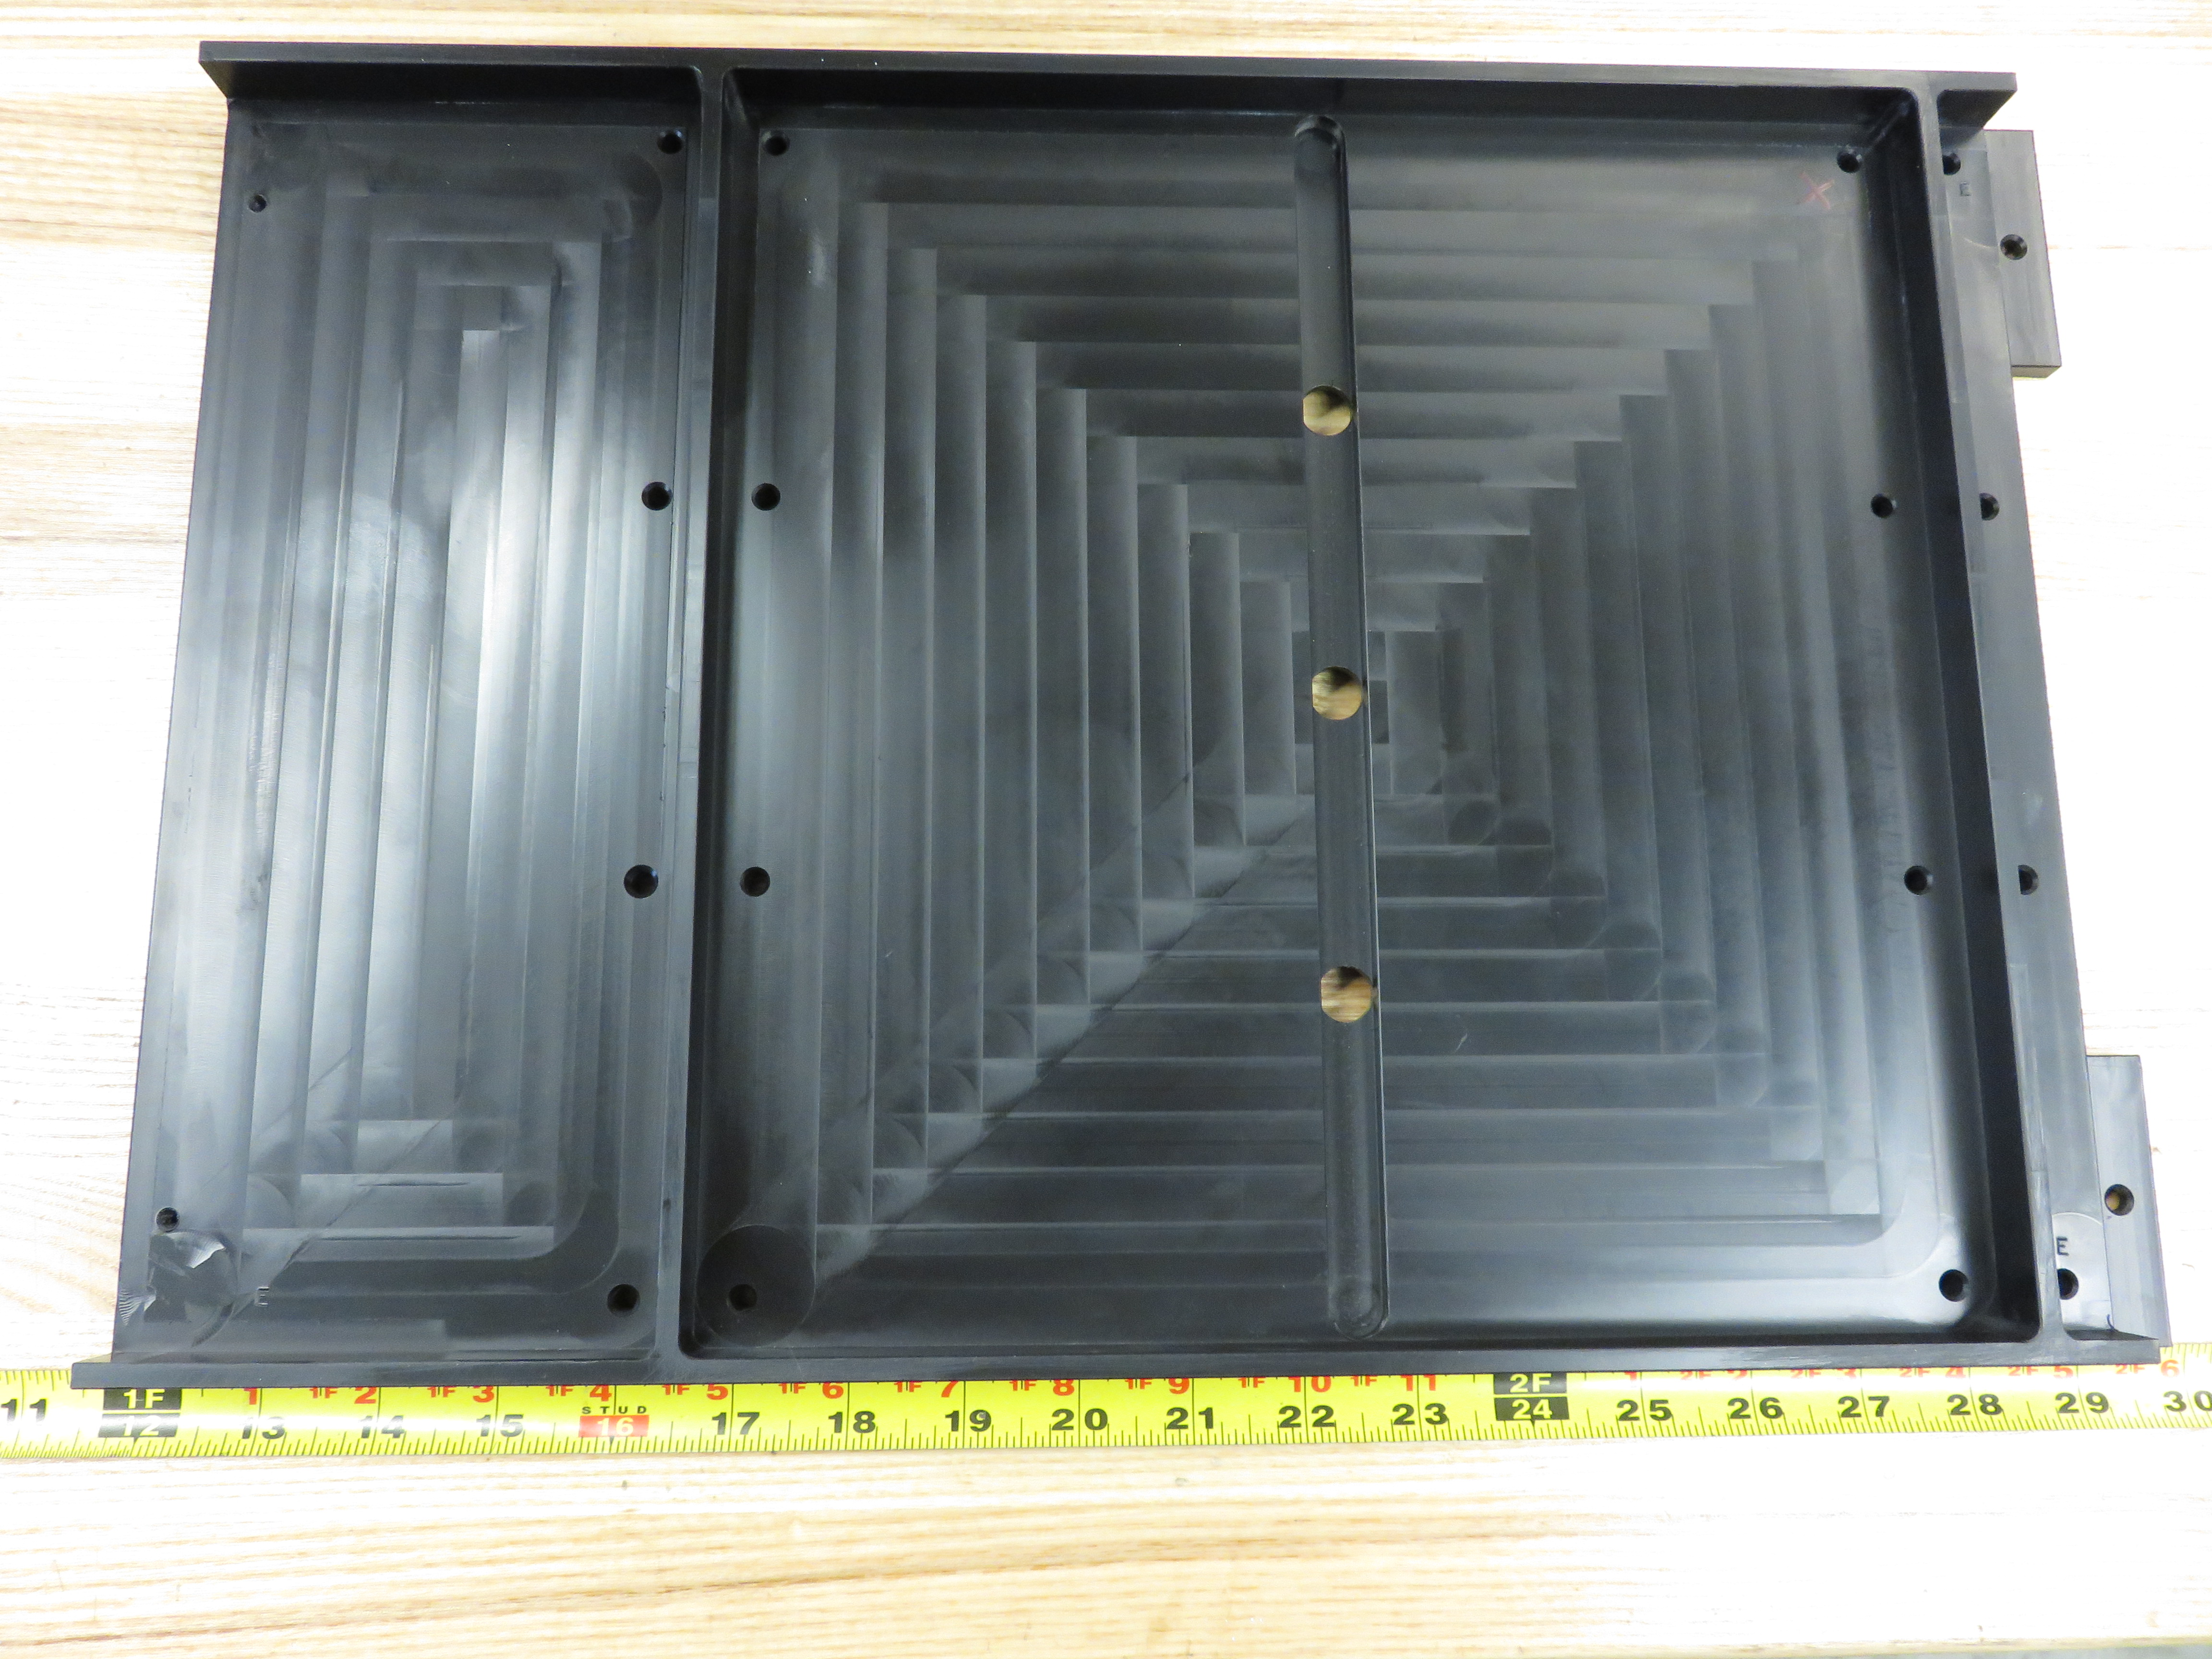
\includegraphics[scale=0.1]{facility/MachinedParts/E_meas_v2.JPG}}}
  \end{center}
\caption{(a) insulation (b) frame. } 
\label{fig:partsE}
\end{figure}

\begin{figure}[h!]
  \begin{center}
  {\subfigcapskip = 5pt \subfigcapmargin = -12pt \subfigure[]{\label{fig:edge-a}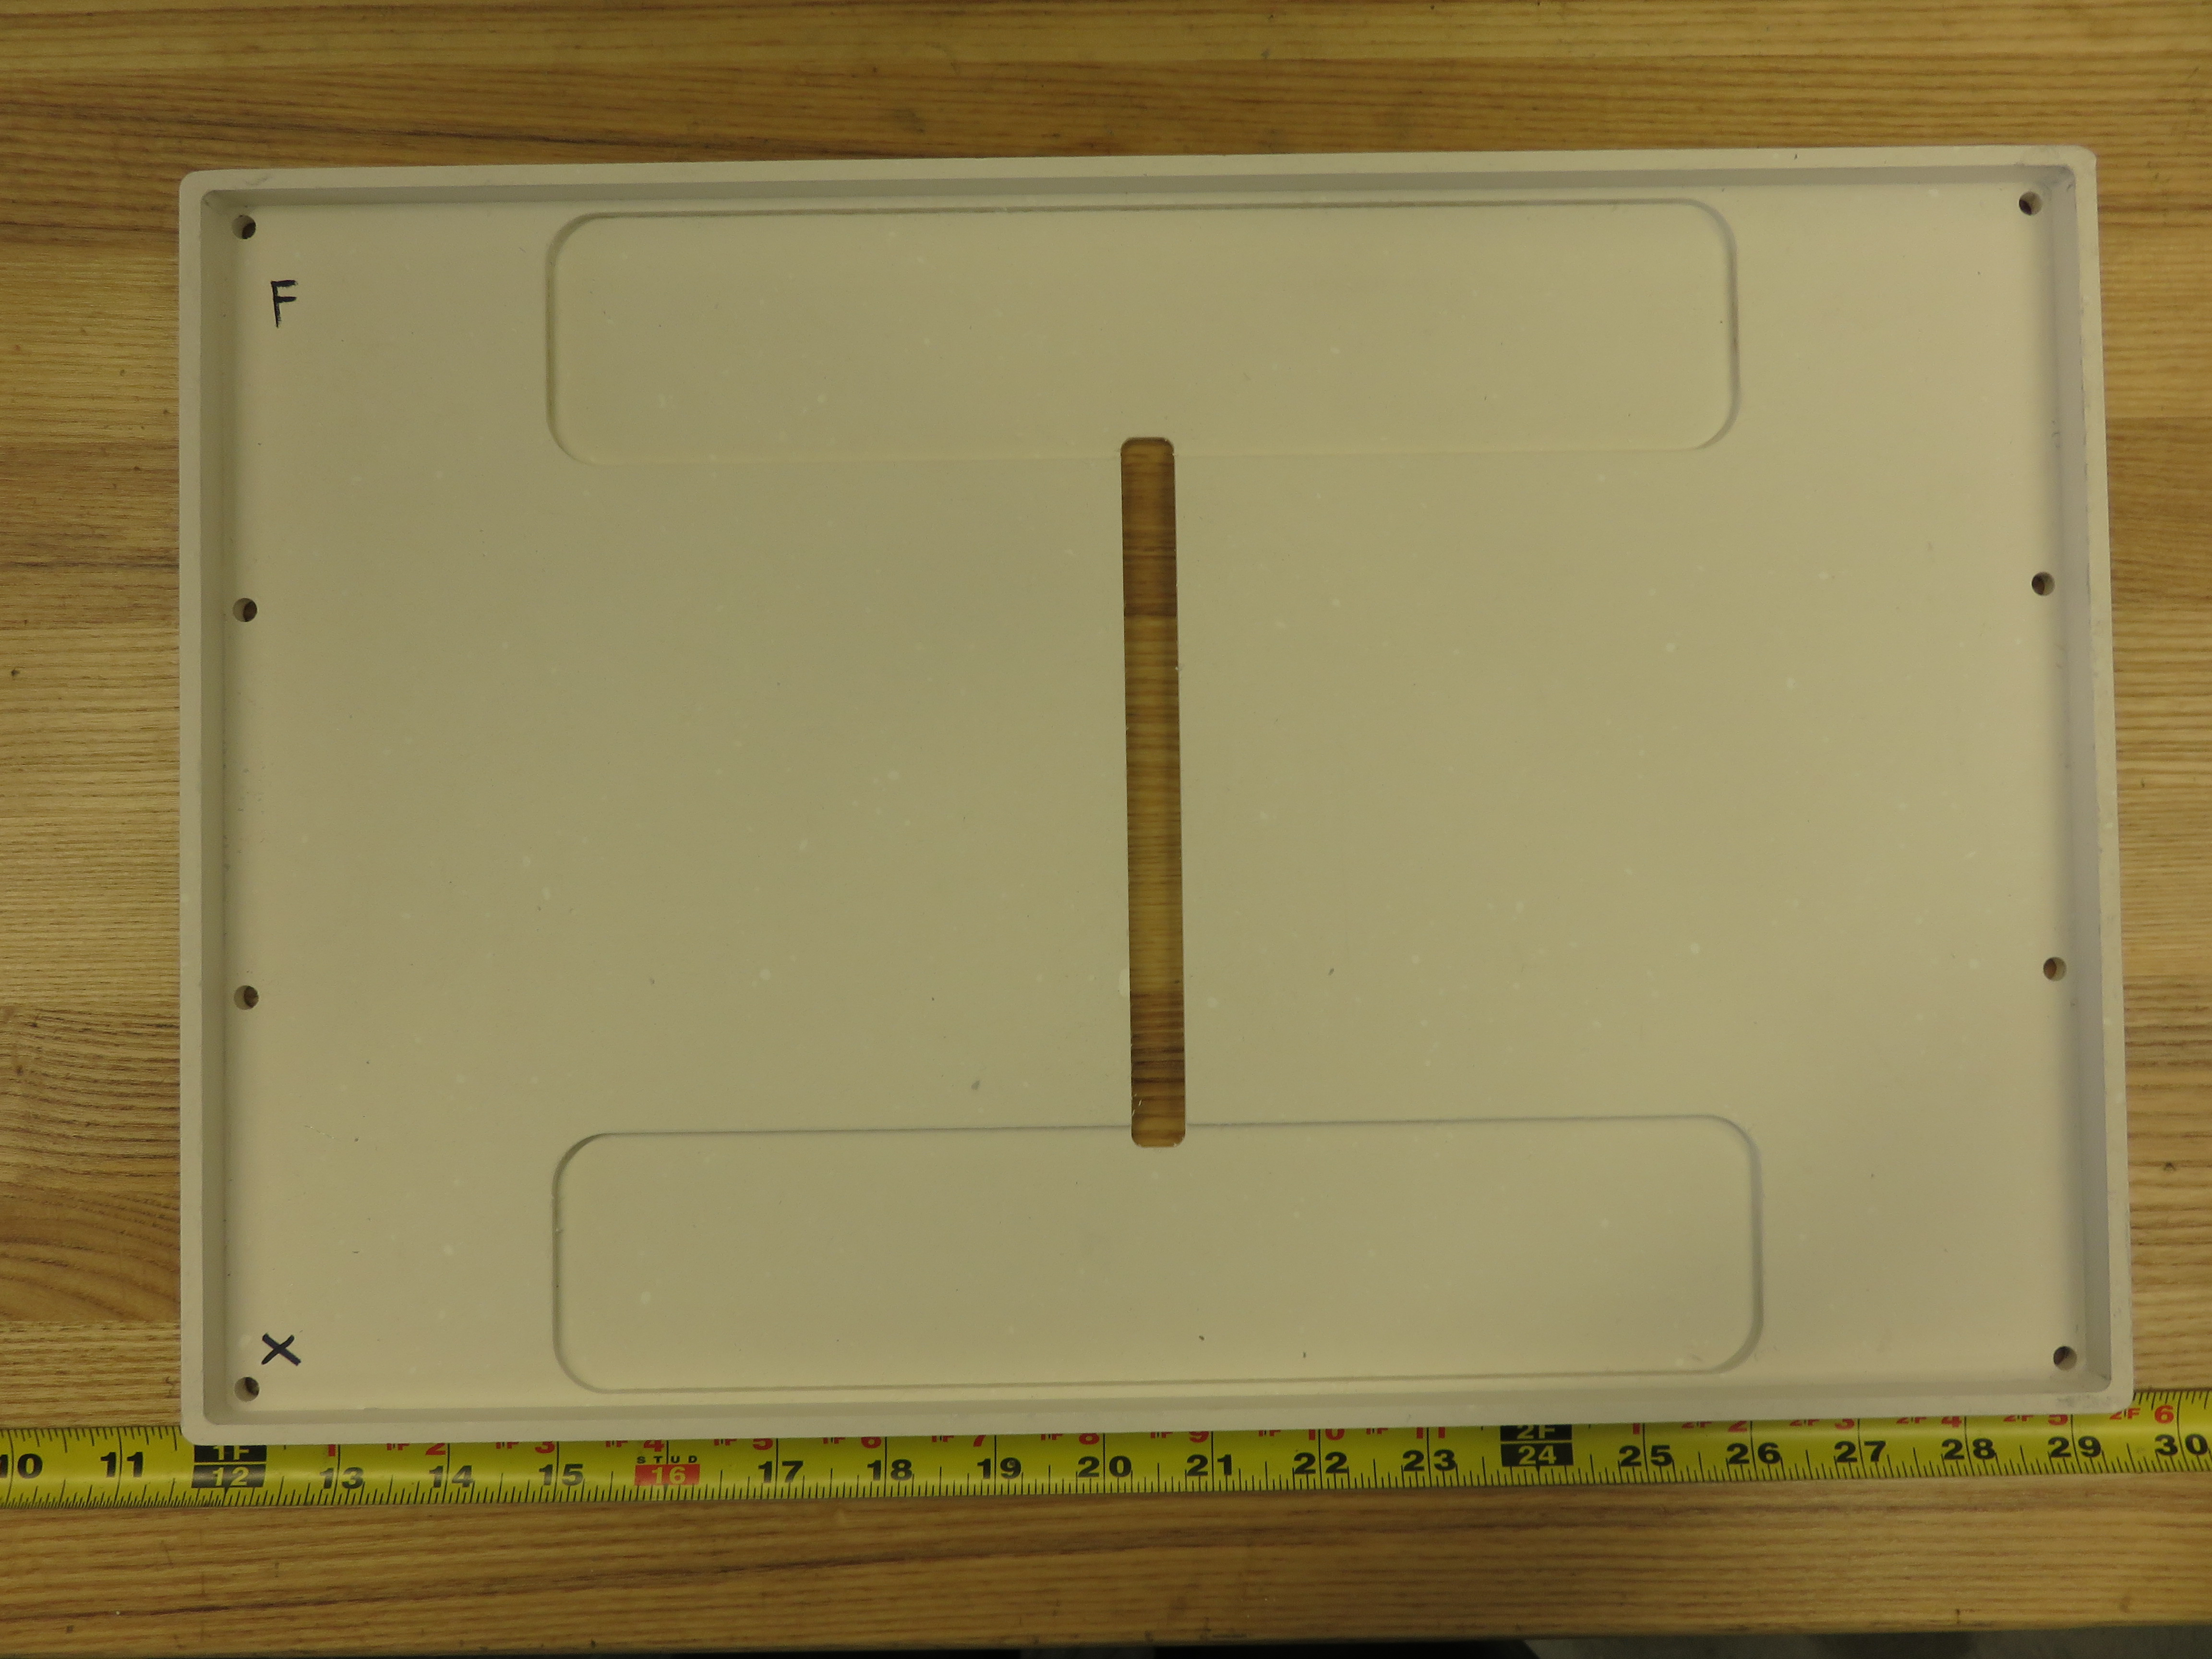
\includegraphics[scale=0.1]{facility/MachinedParts/F_insul_v2.JPG}}}
   {\subfigcapskip = 5pt \subfigcapmargin = -12pt  \subfigure[]{\label{fig:edge-b}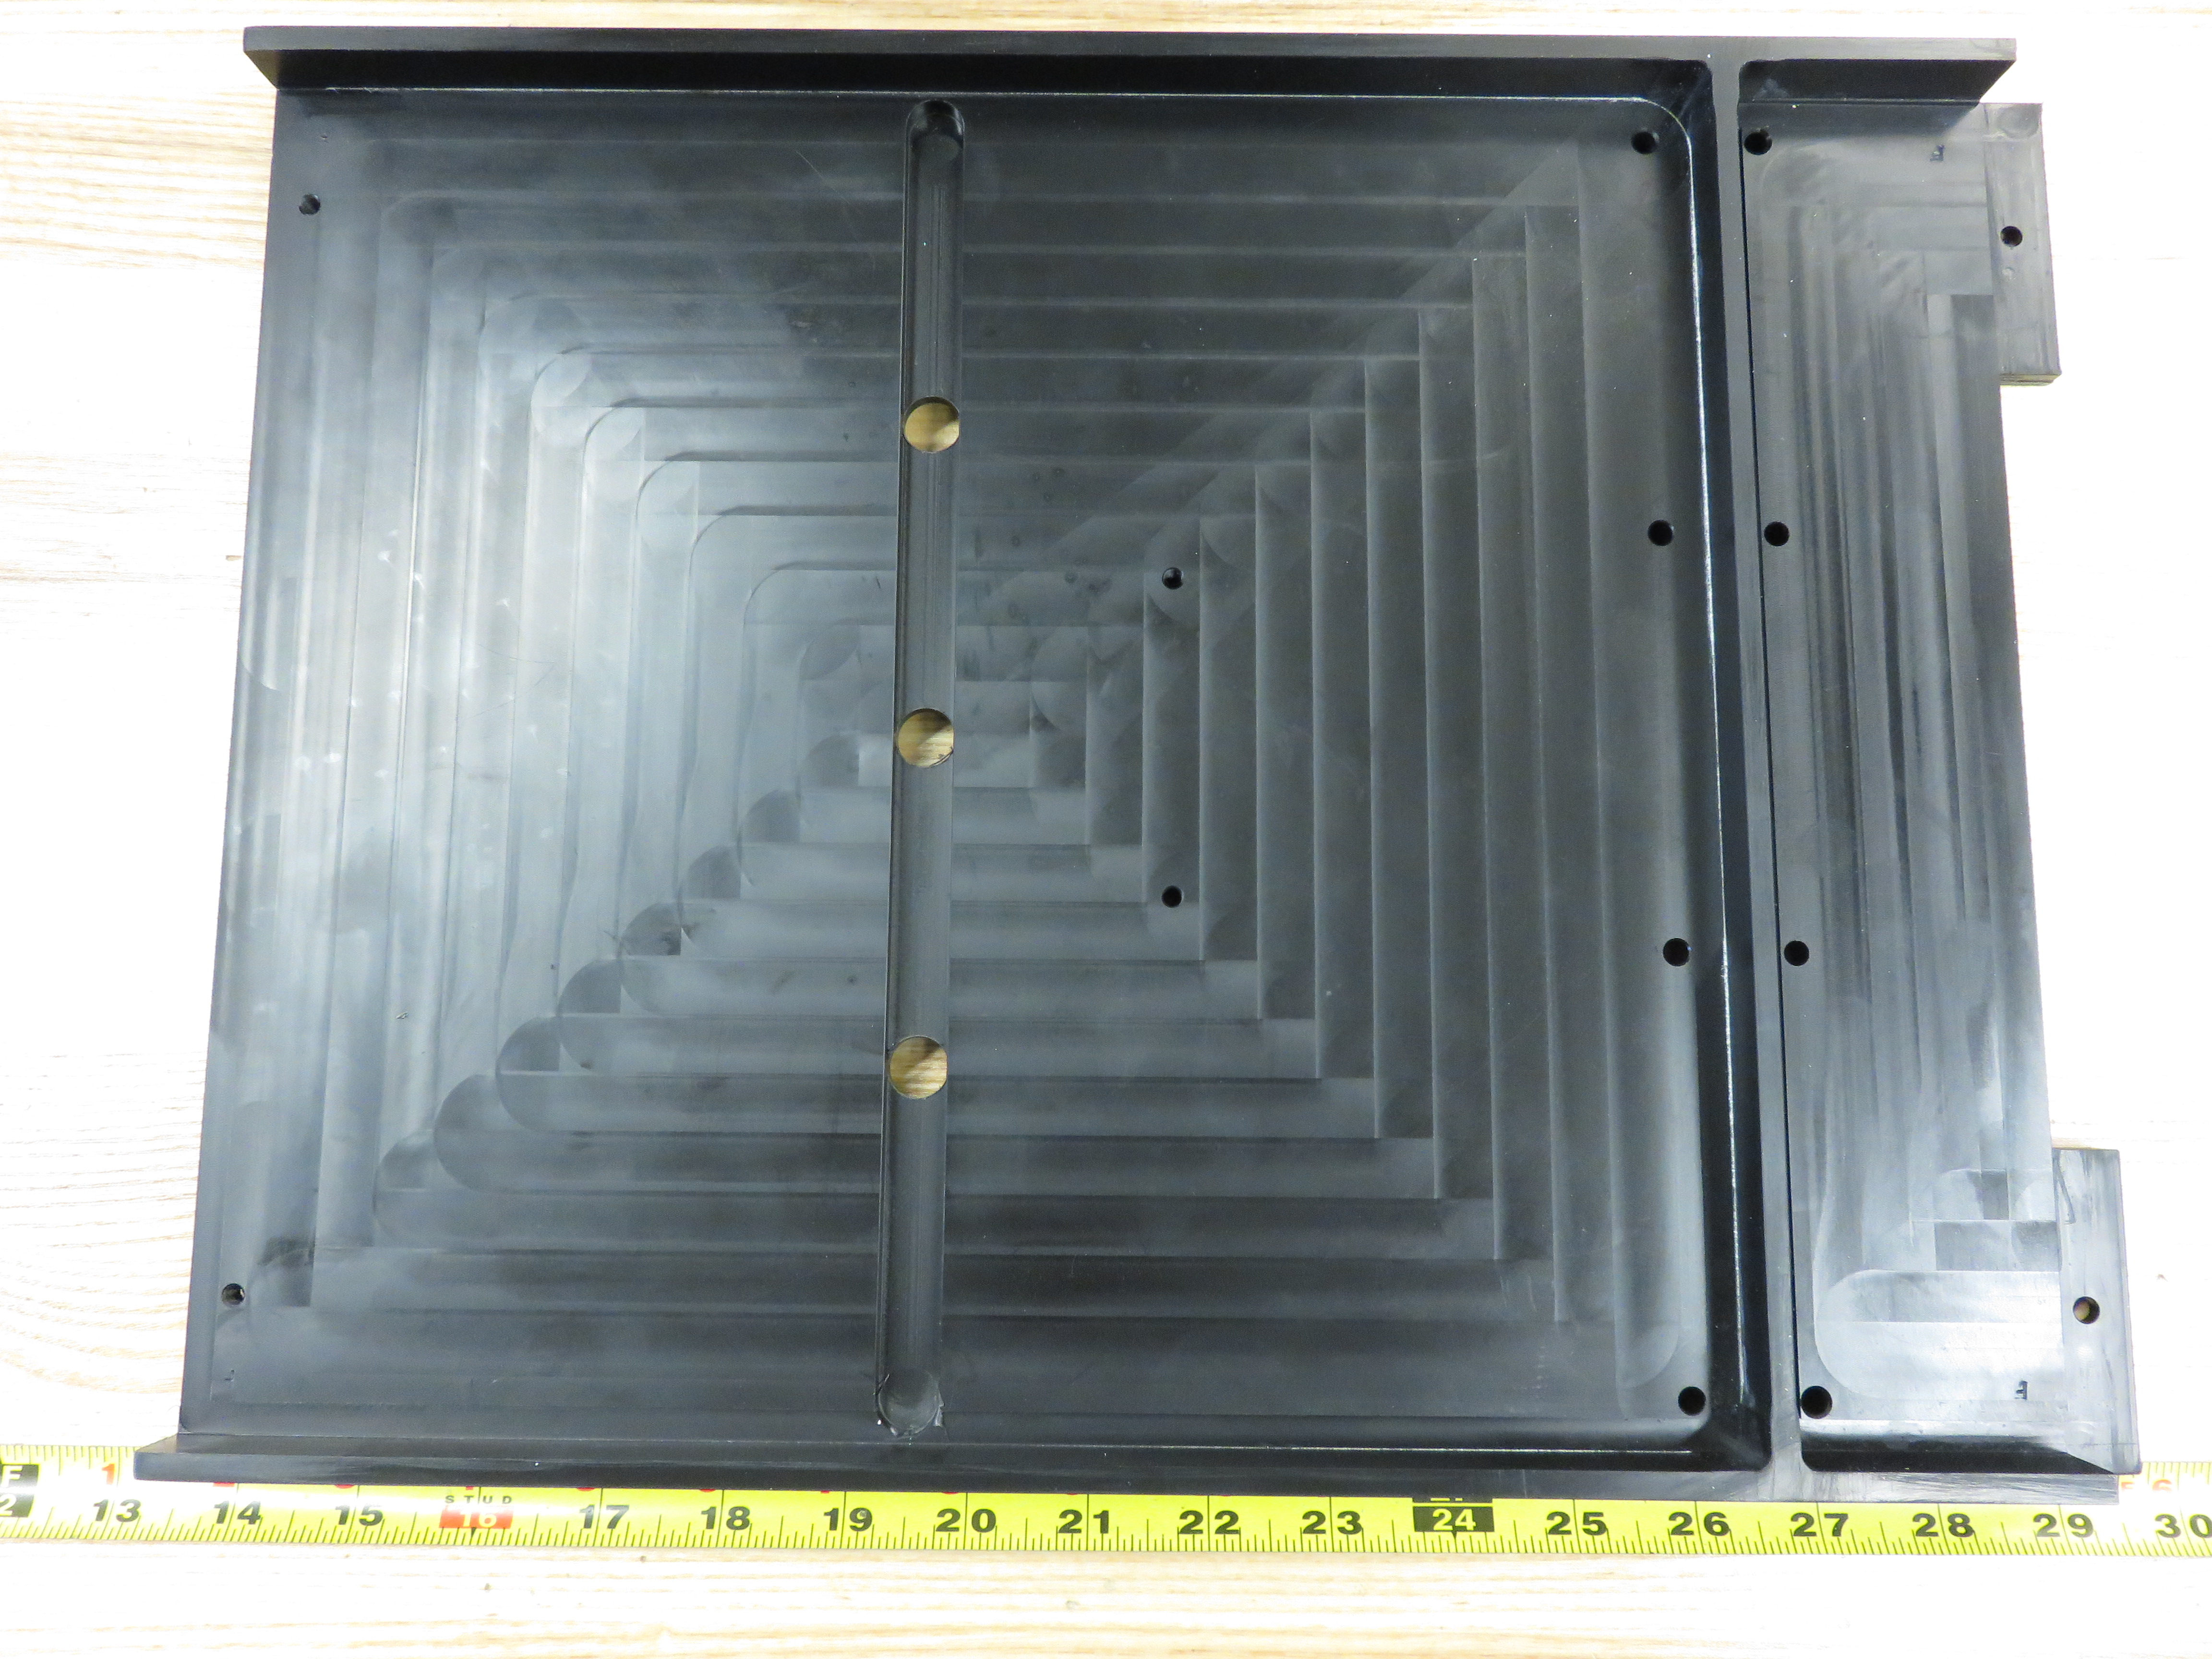
\includegraphics[scale=0.1]{facility/MachinedParts/F_meas_v1.JPG}}}
  \end{center}
\caption{(a) insulation (b) frame. } 
\label{fig:partsF}
\end{figure}

\begin{figure}[h!]
\centering
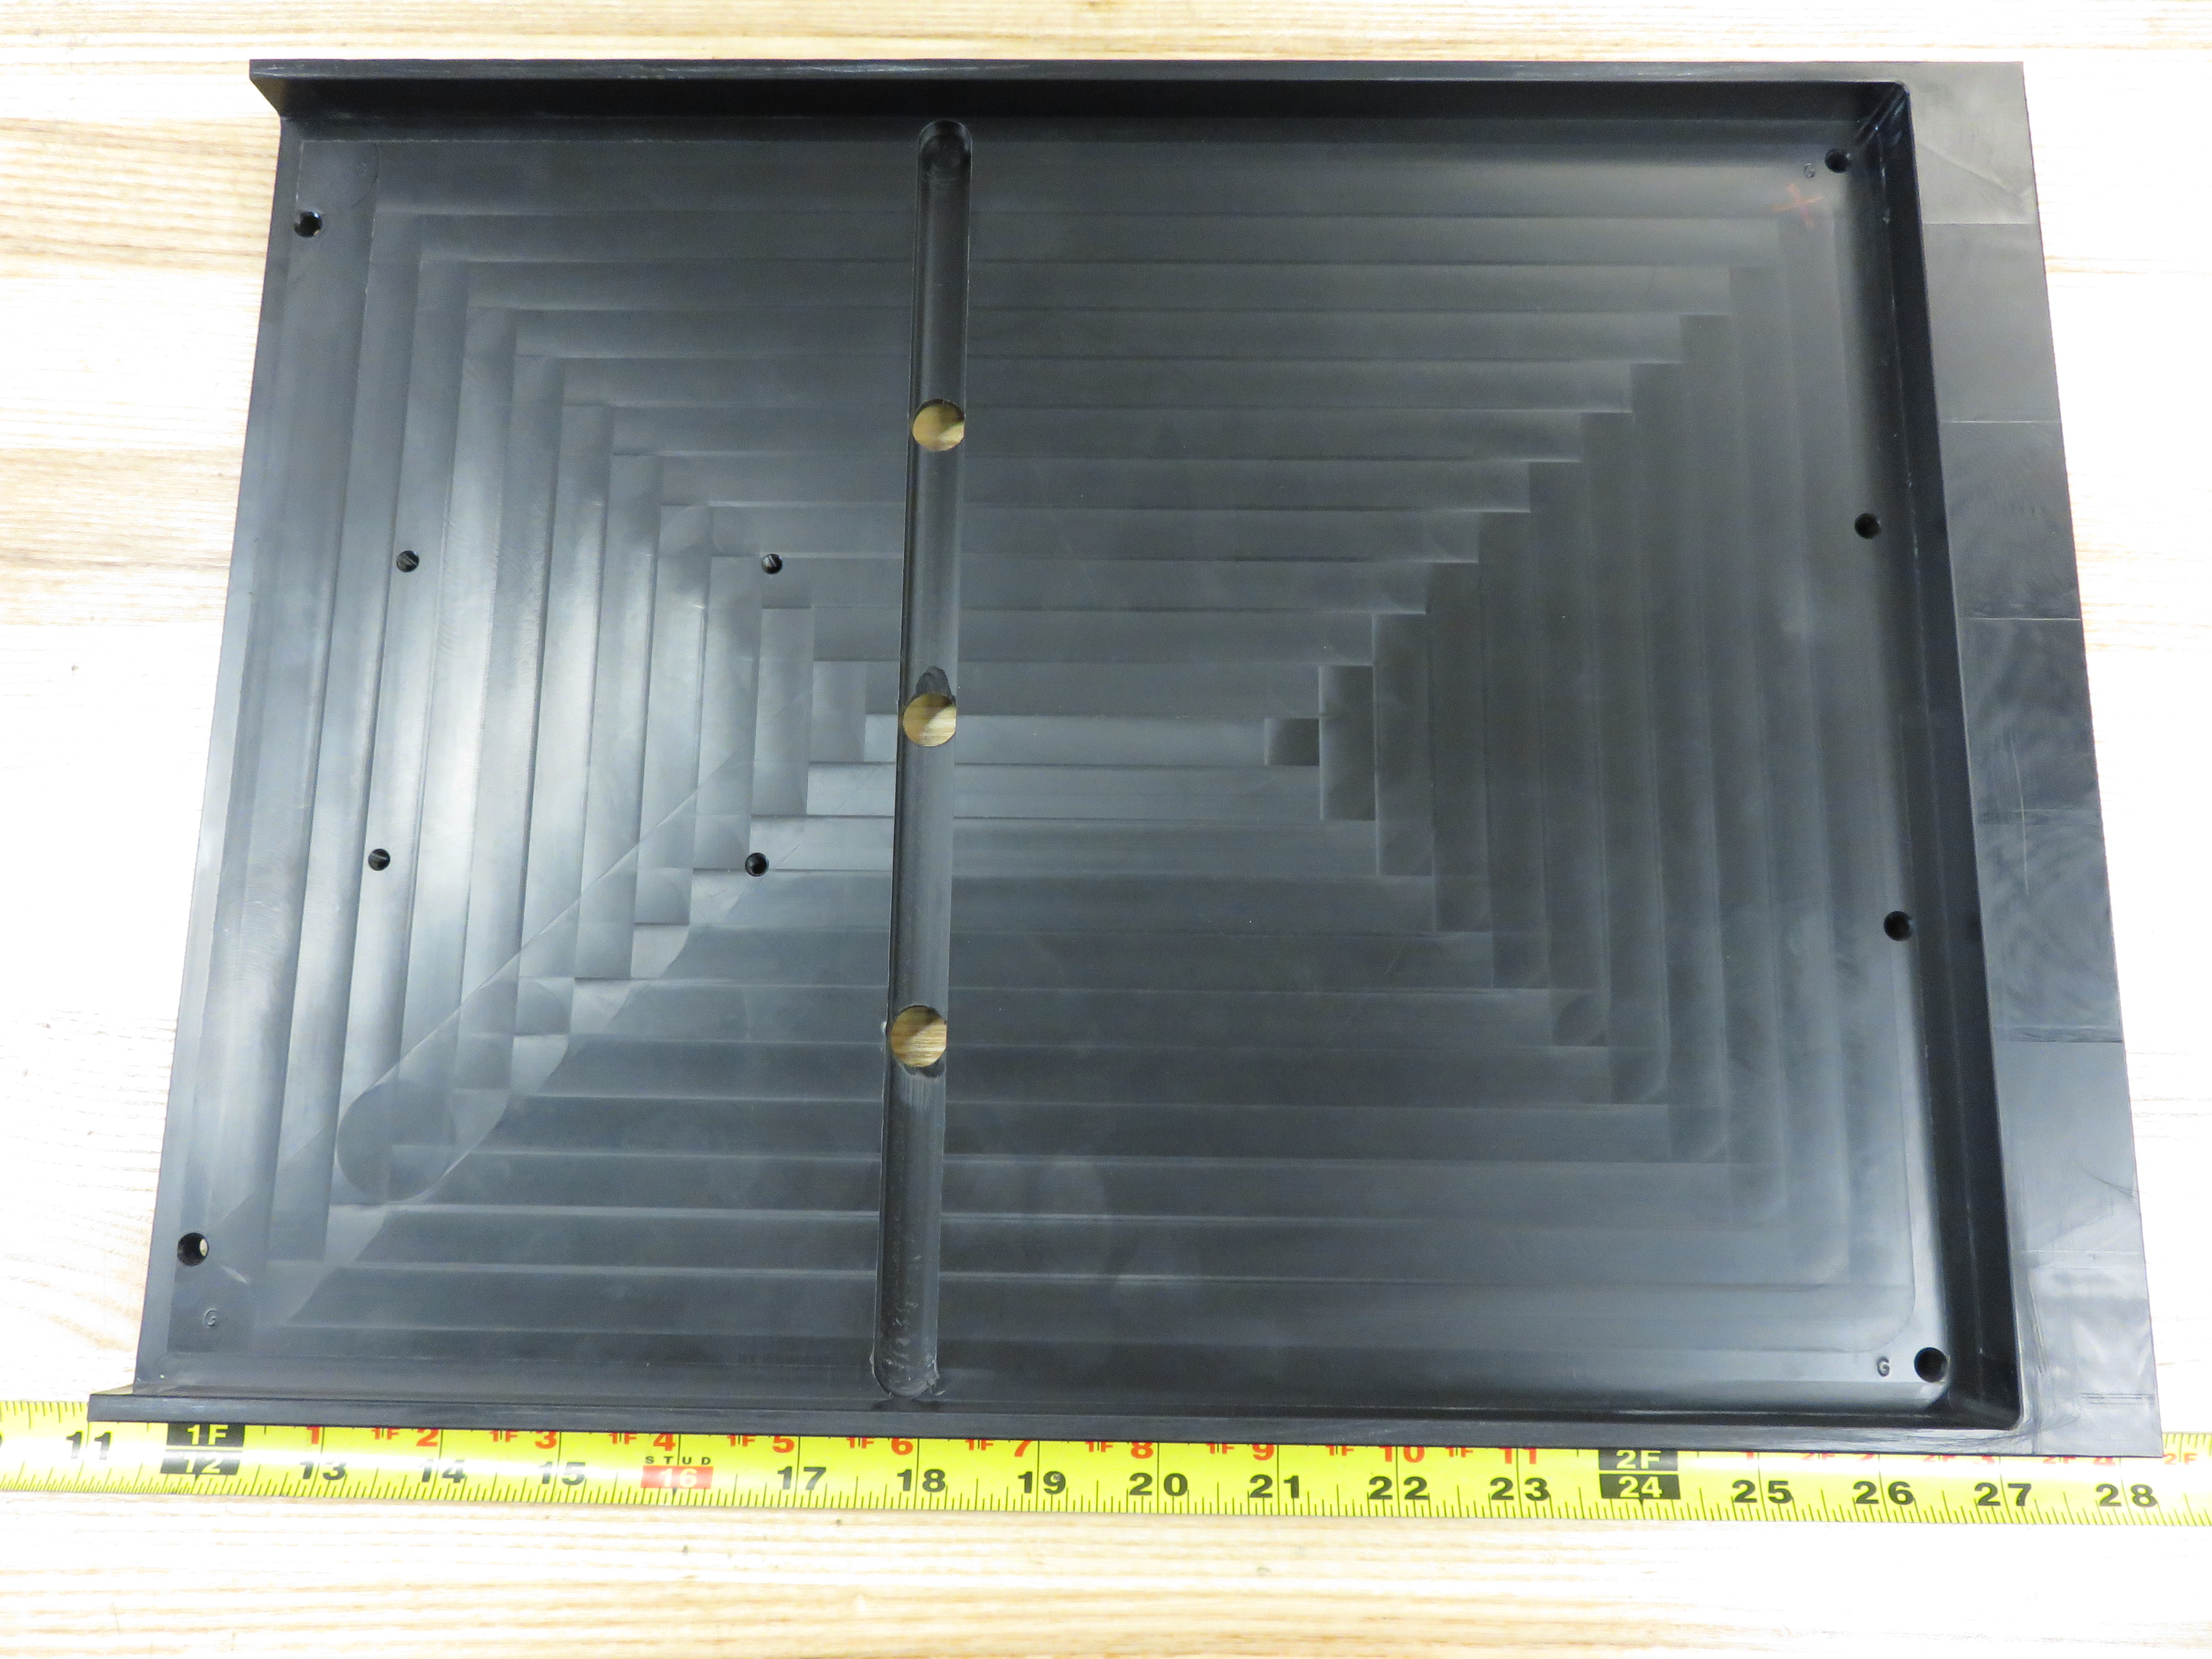
\includegraphics[scale=0.1]{facility/MachinedParts/G_meas_v2.JPG}
\caption{ \footnotesize part}
\label{fig:partsG}
\end{figure}
